\documentclass[11pt]{article}

%----------------------------------------------------------------------------------------
%	MIO
%----------------------------------------------------------------------------------------

% Comandos propios

\setlength{\hoffset}{-0.5cm}
\setlength{\voffset}{-1.5cm}
\setlength{\textwidth}{18.5cm}
\setlength{\textheight}{25.5cm}
\setlength{\parskip}{0pt}
\setlength{\parindent}{0in}

\usepackage{mathtools}
\usepackage[framemethod=TikZ]{mdframed} % Para entorno enunciado
\usepackage{dsfont}
\DeclarePairedDelimiter\abs{\lvert}{\rvert}%
\usepackage{cancel}
\usepackage{blindtext} % Package to generate dummy text
\usepackage{charter} % Use the Charter font
\usepackage[utf8]{inputenc} % Use UTF-8 encoding
\usepackage{microtype} % Slightly tweak font spacing for aesthetics
\usepackage[english]{babel} % Language hyphenation and typographical rules
\usepackage{amsthm, amsmath, amssymb} % Mathematical typesetting
\usepackage{float} % Improved interface for floating objects
\usepackage[final, colorlinks = true, 
linkcolor = black, 
citecolor = black]{hyperref} % For hyperlinks in the PDF
\usepackage{graphicx, multicol} % Enhanced support for graphics
\usepackage{xcolor} % Driver-independent color extensions
\usepackage{marvosym, wasysym} % More symbols
\usepackage{rotating} % Rotation tools
\usepackage{censor} % Facilities for controlling restricted text
\usepackage{listings} % Environment for non-formatted code, !uses style file!
\usepackage{pseudocode} % Environment for specifying algorithms in a natural way
% Environment for f-structures, !uses style file!
\usepackage{booktabs} % Enhances quality of tables
\usepackage{tikz-qtree} % Easy tree drawing tool
% Configuration for b-trees and b+-trees, !uses style file!
%\usepackage[backend=biber,style=numeric,
%            sorting=nyt]{biblatex} % Complete reimplementation of bibliographic facilities
%\addbibresource{ecl.bib}
\usepackage{csquotes} % Context sensitive quotation facilities
\usepackage[yyyymmdd]{datetime} % Uses YEAR-MONTH-DAY format for dates
\renewcommand{\dateseparator}{-} % Sets dateseparator to '-'
\usepackage{fancyhdr} % Headers and footers
\pagestyle{fancy} % All pages have headers and footers
\fancyhead{}\renewcommand{\headrulewidth}{0pt} % Blank out the default header
\fancyfoot[L]{} % Custom footer text
\fancyfoot[C]{} % Custom footer text
\fancyfoot[R]{\thepage} % Custom footer text
\newcommand{\note}[1]{\marginpar{\scriptsize \textcolor{red}{#1}}} % Enables comments in red on margin



\usepackage[T1]{fontenc}
\usepackage{graphicx}
\usepackage{grffile}
\usepackage{longtable}
\usepackage{wrapfig}
\usepackage{rotating}
\usepackage[normalem]{ulem}
\usepackage{amsmath}
\usepackage{textcomp}
\usepackage{amssymb}
\usepackage{listings}
\usepackage{capt-of}
\usepackage{hyperref}
\hypersetup{colorlinks=true, linkcolor=black}
\setlength{\parindent}{0in}
\usepackage[margin=1.1in]{geometry}
\usepackage[spanish]{babel}
\usepackage{mathtools}
\usepackage{palatino}
\usepackage{fancyhdr}
\usepackage{sectsty}
\usepackage{engord}
\usepackage{cite}
\usepackage{graphicx}
\usepackage{setspace}
\usepackage[compact]{titlesec}
\usepackage[center]{caption}
\usepackage{placeins}
\usepackage{tikz}
\usetikzlibrary{positioning}
\usetikzlibrary{bayesnet}
\usetikzlibrary{shapes.geometric}
\usetikzlibrary{decorations.text}
\usepackage{color}
\usepackage{amsmath}
\usepackage{minted}
\usepackage{pdfpages}
\usepackage[framemethod=TikZ]{mdframed} % Para entorno enunciado
\usepackage{amsthm}

\definecolor{myBlue}{rgb}{1, 0.733, 0.612}
\newcommand{\I}{\mathbb{I}}
\newcommand{\la}{\langle}
\newcommand{\ra}{\rangle}
\newcommand{\myparagraph}[1]{\paragraph*{ \\ #1}\mbox{}\\}

\theoremstyle{plain}
\newtheorem*{theorem*}{Teorema}
\newtheorem{theorem}{Teorema}

%%%%%%%%%%%%%%%%%%%%%%%%%%%%%% Entorno para enunciados
%https://texblog.org/2015/09/30/fancy-boxes-for-theorem-lemma-and-proof-with-mdframed/
%\newcounter{enunciado}[section] - para resetear el counter por secciones
\newcounter{enunciado}
\setcounter{enunciado}{0}

% Esta línea pone la numeración de los ejercicios como {seccion}.{ejercicio}
%\renewcommand{\thetheo}{\arabic{section}.\arabic{enunciado}}
\newcommand{\thetheo}{\arabic{enunciado}}

\newenvironment{enunciado}[2][]{%
	\refstepcounter{enunciado}%
	\ifstrempty{#1}%
	{\mdfsetup{%
			frametitle={%
				\tikz[rounded corners, baseline=(current bounding box.east),outer sep=0pt]
				\node[anchor=east,rectangle,fill=myBlue]
				{\strut Ejercicio~\thetheo};}}
	}%
	{\mdfsetup{%
			frametitle={%
				\tikz[rounded corners, baseline=(current bounding box.east),outer sep=0pt]
				\node[anchor=east,rectangle,fill=myBlue]
				{\strut Ejercicio~\thetheo:~#1};}}%
	}%
	\mdfsetup{roundcorner=5pt, innertopmargin=10pt,linecolor=myBlue,%
		linewidth=2pt,topline=true,%
		frametitleaboveskip=\dimexpr-\ht\strutbox\relax
	}
	\begin{mdframed}[]\relax%
		%\label{#2}
	}
	{\end{mdframed}}
%%%%%%%%%%%%%%%%%%%%%%%%%%%%%%

%----------------------------------------------------------------------------------------
%	NO MIO
%----------------------------------------------------------------------------------------

    \usepackage[breakable]{tcolorbox}
    \usepackage{parskip} % Stop auto-indenting (to mimic markdown behaviour)
    
    \usepackage{iftex}
    \ifPDFTeX
    	\usepackage[T1]{fontenc}
    	\usepackage{mathpazo}
    \else
    	\usepackage{fontspec}
    \fi

    % Basic figure setup, for now with no caption control since it's done
    % automatically by Pandoc (which extracts ![](path) syntax from Markdown).
    \usepackage{graphicx}
    % Maintain compatibility with old templates. Remove in nbconvert 6.0
    \let\Oldincludegraphics\includegraphics
    % Ensure that by default, figures have no caption (until we provide a
    % proper Figure object with a Caption API and a way to capture that
    % in the conversion process - todo).
    \usepackage{caption}
    \DeclareCaptionFormat{nocaption}{}
    \captionsetup{format=nocaption,aboveskip=0pt,belowskip=0pt}

    \usepackage{float}
    \floatplacement{figure}{H} % forces figures to be placed at the correct location
    \usepackage{xcolor} % Allow colors to be defined
    \usepackage{enumerate} % Needed for markdown enumerations to work
    \usepackage{geometry} % Used to adjust the document margins
    \usepackage{amsmath} % Equations
    \usepackage{amssymb} % Equations
    \usepackage{textcomp} % defines textquotesingle
    % Hack from http://tex.stackexchange.com/a/47451/13684:
    \AtBeginDocument{%
        \def\PYZsq{\textquotesingle}% Upright quotes in Pygmentized code
    }
    \usepackage{upquote} % Upright quotes for verbatim code
    \usepackage{eurosym} % defines \euro
    \usepackage[mathletters]{ucs} % Extended unicode (utf-8) support
    \usepackage{fancyvrb} % verbatim replacement that allows latex
    \usepackage{grffile} % extends the file name processing of package graphics 
                         % to support a larger range
    \makeatletter % fix for old versions of grffile with XeLaTeX
    \@ifpackagelater{grffile}{2019/11/01}
    {
      % Do nothing on new versions
    }
    {
      \def\Gread@@xetex#1{%
        \IfFileExists{"\Gin@base".bb}%
        {\Gread@eps{\Gin@base.bb}}%
        {\Gread@@xetex@aux#1}%
      }
    }
    \makeatother
    \usepackage[Export]{adjustbox} % Used to constrain images to a maximum size
    \adjustboxset{max size={0.9\linewidth}{0.9\paperheight}}

    % The hyperref package gives us a pdf with properly built
    % internal navigation ('pdf bookmarks' for the table of contents,
    % internal cross-reference links, web links for URLs, etc.)
    \usepackage{hyperref}
    % The default LaTeX title has an obnoxious amount of whitespace. By default,
    % titling removes some of it. It also provides customization options.
    \usepackage{titling}
    \usepackage{longtable} % longtable support required by pandoc >1.10
    \usepackage{booktabs}  % table support for pandoc > 1.12.2
    \usepackage[inline]{enumitem} % IRkernel/repr support (it uses the enumerate* environment)
    \usepackage[normalem]{ulem} % ulem is needed to support strikethroughs (\sout)
                                % normalem makes italics be italics, not underlines
    \usepackage{mathrsfs}
    

    
    % Colors for the hyperref package
    \definecolor{urlcolor}{rgb}{0,.145,.698}
    \definecolor{linkcolor}{rgb}{.71,0.21,0.01}
    \definecolor{citecolor}{rgb}{.12,.54,.11}

    % ANSI colors
    \definecolor{ansi-black}{HTML}{3E424D}
    \definecolor{ansi-black-intense}{HTML}{282C36}
    \definecolor{ansi-red}{HTML}{E75C58}
    \definecolor{ansi-red-intense}{HTML}{B22B31}
    \definecolor{ansi-green}{HTML}{00A250}
    \definecolor{ansi-green-intense}{HTML}{007427}
    \definecolor{ansi-yellow}{HTML}{DDB62B}
    \definecolor{ansi-yellow-intense}{HTML}{B27D12}
    \definecolor{ansi-blue}{HTML}{208FFB}
    \definecolor{ansi-blue-intense}{HTML}{0065CA}
    \definecolor{ansi-magenta}{HTML}{D160C4}
    \definecolor{ansi-magenta-intense}{HTML}{A03196}
    \definecolor{ansi-cyan}{HTML}{60C6C8}
    \definecolor{ansi-cyan-intense}{HTML}{258F8F}
    \definecolor{ansi-white}{HTML}{C5C1B4}
    \definecolor{ansi-white-intense}{HTML}{A1A6B2}
    \definecolor{ansi-default-inverse-fg}{HTML}{FFFFFF}
    \definecolor{ansi-default-inverse-bg}{HTML}{000000}

    % common color for the border for error outputs.
    \definecolor{outerrorbackground}{HTML}{FFDFDF}

    % commands and environments needed by pandoc snippets
    % extracted from the output of `pandoc -s`
    \providecommand{\tightlist}{%
      \setlength{\itemsep}{0pt}\setlength{\parskip}{0pt}}
    \DefineVerbatimEnvironment{Highlighting}{Verbatim}{commandchars=\\\{\}}
    % Add ',fontsize=\small' for more characters per line
    \newenvironment{Shaded}{}{}
    \newcommand{\KeywordTok}[1]{\textcolor[rgb]{0.00,0.44,0.13}{\textbf{{#1}}}}
    \newcommand{\DataTypeTok}[1]{\textcolor[rgb]{0.56,0.13,0.00}{{#1}}}
    \newcommand{\DecValTok}[1]{\textcolor[rgb]{0.25,0.63,0.44}{{#1}}}
    \newcommand{\BaseNTok}[1]{\textcolor[rgb]{0.25,0.63,0.44}{{#1}}}
    \newcommand{\FloatTok}[1]{\textcolor[rgb]{0.25,0.63,0.44}{{#1}}}
    \newcommand{\CharTok}[1]{\textcolor[rgb]{0.25,0.44,0.63}{{#1}}}
    \newcommand{\StringTok}[1]{\textcolor[rgb]{0.25,0.44,0.63}{{#1}}}
    \newcommand{\CommentTok}[1]{\textcolor[rgb]{0.38,0.63,0.69}{\textit{{#1}}}}
    \newcommand{\OtherTok}[1]{\textcolor[rgb]{0.00,0.44,0.13}{{#1}}}
    \newcommand{\AlertTok}[1]{\textcolor[rgb]{1.00,0.00,0.00}{\textbf{{#1}}}}
    \newcommand{\FunctionTok}[1]{\textcolor[rgb]{0.02,0.16,0.49}{{#1}}}
    \newcommand{\RegionMarkerTok}[1]{{#1}}
    \newcommand{\ErrorTok}[1]{\textcolor[rgb]{1.00,0.00,0.00}{\textbf{{#1}}}}
    \newcommand{\NormalTok}[1]{{#1}}
    
    % Additional commands for more recent versions of Pandoc
    \newcommand{\ConstantTok}[1]{\textcolor[rgb]{0.53,0.00,0.00}{{#1}}}
    \newcommand{\SpecialCharTok}[1]{\textcolor[rgb]{0.25,0.44,0.63}{{#1}}}
    \newcommand{\VerbatimStringTok}[1]{\textcolor[rgb]{0.25,0.44,0.63}{{#1}}}
    \newcommand{\SpecialStringTok}[1]{\textcolor[rgb]{0.73,0.40,0.53}{{#1}}}
    \newcommand{\ImportTok}[1]{{#1}}
    \newcommand{\DocumentationTok}[1]{\textcolor[rgb]{0.73,0.13,0.13}{\textit{{#1}}}}
    \newcommand{\AnnotationTok}[1]{\textcolor[rgb]{0.38,0.63,0.69}{\textbf{\textit{{#1}}}}}
    \newcommand{\CommentVarTok}[1]{\textcolor[rgb]{0.38,0.63,0.69}{\textbf{\textit{{#1}}}}}
    \newcommand{\VariableTok}[1]{\textcolor[rgb]{0.10,0.09,0.49}{{#1}}}
    \newcommand{\ControlFlowTok}[1]{\textcolor[rgb]{0.00,0.44,0.13}{\textbf{{#1}}}}
    \newcommand{\OperatorTok}[1]{\textcolor[rgb]{0.40,0.40,0.40}{{#1}}}
    \newcommand{\BuiltInTok}[1]{{#1}}
    \newcommand{\ExtensionTok}[1]{{#1}}
    \newcommand{\PreprocessorTok}[1]{\textcolor[rgb]{0.74,0.48,0.00}{{#1}}}
    \newcommand{\AttributeTok}[1]{\textcolor[rgb]{0.49,0.56,0.16}{{#1}}}
    \newcommand{\InformationTok}[1]{\textcolor[rgb]{0.38,0.63,0.69}{\textbf{\textit{{#1}}}}}
    \newcommand{\WarningTok}[1]{\textcolor[rgb]{0.38,0.63,0.69}{\textbf{\textit{{#1}}}}}
    
    
    % Define a nice break command that doesn't care if a line doesn't already
    % exist.
    \def\br{\hspace*{\fill} \\* }
    % Math Jax compatibility definitions
    \def\gt{>}
    \def\lt{<}
    \let\Oldtex\TeX
    \let\Oldlatex\LaTeX
    \renewcommand{\TeX}{\textrm{\Oldtex}}
    \renewcommand{\LaTeX}{\textrm{\Oldlatex}}
    % Document parameters
    % Document title
    \title{midterm}
    
    
    
    
    
% Pygments definitions
\makeatletter
\def\PY@reset{\let\PY@it=\relax \let\PY@bf=\relax%
    \let\PY@ul=\relax \let\PY@tc=\relax%
    \let\PY@bc=\relax \let\PY@ff=\relax}
\def\PY@tok#1{\csname PY@tok@#1\endcsname}
\def\PY@toks#1+{\ifx\relax#1\empty\else%
    \PY@tok{#1}\expandafter\PY@toks\fi}
\def\PY@do#1{\PY@bc{\PY@tc{\PY@ul{%
    \PY@it{\PY@bf{\PY@ff{#1}}}}}}}
\def\PY#1#2{\PY@reset\PY@toks#1+\relax+\PY@do{#2}}

\expandafter\def\csname PY@tok@w\endcsname{\def\PY@tc##1{\textcolor[rgb]{0.73,0.73,0.73}{##1}}}
\expandafter\def\csname PY@tok@c\endcsname{\let\PY@it=\textit\def\PY@tc##1{\textcolor[rgb]{0.25,0.50,0.50}{##1}}}
\expandafter\def\csname PY@tok@cp\endcsname{\def\PY@tc##1{\textcolor[rgb]{0.74,0.48,0.00}{##1}}}
\expandafter\def\csname PY@tok@k\endcsname{\let\PY@bf=\textbf\def\PY@tc##1{\textcolor[rgb]{0.00,0.50,0.00}{##1}}}
\expandafter\def\csname PY@tok@kp\endcsname{\def\PY@tc##1{\textcolor[rgb]{0.00,0.50,0.00}{##1}}}
\expandafter\def\csname PY@tok@kt\endcsname{\def\PY@tc##1{\textcolor[rgb]{0.69,0.00,0.25}{##1}}}
\expandafter\def\csname PY@tok@o\endcsname{\def\PY@tc##1{\textcolor[rgb]{0.40,0.40,0.40}{##1}}}
\expandafter\def\csname PY@tok@ow\endcsname{\let\PY@bf=\textbf\def\PY@tc##1{\textcolor[rgb]{0.67,0.13,1.00}{##1}}}
\expandafter\def\csname PY@tok@nb\endcsname{\def\PY@tc##1{\textcolor[rgb]{0.00,0.50,0.00}{##1}}}
\expandafter\def\csname PY@tok@nf\endcsname{\def\PY@tc##1{\textcolor[rgb]{0.00,0.00,1.00}{##1}}}
\expandafter\def\csname PY@tok@nc\endcsname{\let\PY@bf=\textbf\def\PY@tc##1{\textcolor[rgb]{0.00,0.00,1.00}{##1}}}
\expandafter\def\csname PY@tok@nn\endcsname{\let\PY@bf=\textbf\def\PY@tc##1{\textcolor[rgb]{0.00,0.00,1.00}{##1}}}
\expandafter\def\csname PY@tok@ne\endcsname{\let\PY@bf=\textbf\def\PY@tc##1{\textcolor[rgb]{0.82,0.25,0.23}{##1}}}
\expandafter\def\csname PY@tok@nv\endcsname{\def\PY@tc##1{\textcolor[rgb]{0.10,0.09,0.49}{##1}}}
\expandafter\def\csname PY@tok@no\endcsname{\def\PY@tc##1{\textcolor[rgb]{0.53,0.00,0.00}{##1}}}
\expandafter\def\csname PY@tok@nl\endcsname{\def\PY@tc##1{\textcolor[rgb]{0.63,0.63,0.00}{##1}}}
\expandafter\def\csname PY@tok@ni\endcsname{\let\PY@bf=\textbf\def\PY@tc##1{\textcolor[rgb]{0.60,0.60,0.60}{##1}}}
\expandafter\def\csname PY@tok@na\endcsname{\def\PY@tc##1{\textcolor[rgb]{0.49,0.56,0.16}{##1}}}
\expandafter\def\csname PY@tok@nt\endcsname{\let\PY@bf=\textbf\def\PY@tc##1{\textcolor[rgb]{0.00,0.50,0.00}{##1}}}
\expandafter\def\csname PY@tok@nd\endcsname{\def\PY@tc##1{\textcolor[rgb]{0.67,0.13,1.00}{##1}}}
\expandafter\def\csname PY@tok@s\endcsname{\def\PY@tc##1{\textcolor[rgb]{0.73,0.13,0.13}{##1}}}
\expandafter\def\csname PY@tok@sd\endcsname{\let\PY@it=\textit\def\PY@tc##1{\textcolor[rgb]{0.73,0.13,0.13}{##1}}}
\expandafter\def\csname PY@tok@si\endcsname{\let\PY@bf=\textbf\def\PY@tc##1{\textcolor[rgb]{0.73,0.40,0.53}{##1}}}
\expandafter\def\csname PY@tok@se\endcsname{\let\PY@bf=\textbf\def\PY@tc##1{\textcolor[rgb]{0.73,0.40,0.13}{##1}}}
\expandafter\def\csname PY@tok@sr\endcsname{\def\PY@tc##1{\textcolor[rgb]{0.73,0.40,0.53}{##1}}}
\expandafter\def\csname PY@tok@ss\endcsname{\def\PY@tc##1{\textcolor[rgb]{0.10,0.09,0.49}{##1}}}
\expandafter\def\csname PY@tok@sx\endcsname{\def\PY@tc##1{\textcolor[rgb]{0.00,0.50,0.00}{##1}}}
\expandafter\def\csname PY@tok@m\endcsname{\def\PY@tc##1{\textcolor[rgb]{0.40,0.40,0.40}{##1}}}
\expandafter\def\csname PY@tok@gh\endcsname{\let\PY@bf=\textbf\def\PY@tc##1{\textcolor[rgb]{0.00,0.00,0.50}{##1}}}
\expandafter\def\csname PY@tok@gu\endcsname{\let\PY@bf=\textbf\def\PY@tc##1{\textcolor[rgb]{0.50,0.00,0.50}{##1}}}
\expandafter\def\csname PY@tok@gd\endcsname{\def\PY@tc##1{\textcolor[rgb]{0.63,0.00,0.00}{##1}}}
\expandafter\def\csname PY@tok@gi\endcsname{\def\PY@tc##1{\textcolor[rgb]{0.00,0.63,0.00}{##1}}}
\expandafter\def\csname PY@tok@gr\endcsname{\def\PY@tc##1{\textcolor[rgb]{1.00,0.00,0.00}{##1}}}
\expandafter\def\csname PY@tok@ge\endcsname{\let\PY@it=\textit}
\expandafter\def\csname PY@tok@gs\endcsname{\let\PY@bf=\textbf}
\expandafter\def\csname PY@tok@gp\endcsname{\let\PY@bf=\textbf\def\PY@tc##1{\textcolor[rgb]{0.00,0.00,0.50}{##1}}}
\expandafter\def\csname PY@tok@go\endcsname{\def\PY@tc##1{\textcolor[rgb]{0.53,0.53,0.53}{##1}}}
\expandafter\def\csname PY@tok@gt\endcsname{\def\PY@tc##1{\textcolor[rgb]{0.00,0.27,0.87}{##1}}}
\expandafter\def\csname PY@tok@err\endcsname{\def\PY@bc##1{\setlength{\fboxsep}{0pt}\fcolorbox[rgb]{1.00,0.00,0.00}{1,1,1}{\strut ##1}}}
\expandafter\def\csname PY@tok@kc\endcsname{\let\PY@bf=\textbf\def\PY@tc##1{\textcolor[rgb]{0.00,0.50,0.00}{##1}}}
\expandafter\def\csname PY@tok@kd\endcsname{\let\PY@bf=\textbf\def\PY@tc##1{\textcolor[rgb]{0.00,0.50,0.00}{##1}}}
\expandafter\def\csname PY@tok@kn\endcsname{\let\PY@bf=\textbf\def\PY@tc##1{\textcolor[rgb]{0.00,0.50,0.00}{##1}}}
\expandafter\def\csname PY@tok@kr\endcsname{\let\PY@bf=\textbf\def\PY@tc##1{\textcolor[rgb]{0.00,0.50,0.00}{##1}}}
\expandafter\def\csname PY@tok@bp\endcsname{\def\PY@tc##1{\textcolor[rgb]{0.00,0.50,0.00}{##1}}}
\expandafter\def\csname PY@tok@fm\endcsname{\def\PY@tc##1{\textcolor[rgb]{0.00,0.00,1.00}{##1}}}
\expandafter\def\csname PY@tok@vc\endcsname{\def\PY@tc##1{\textcolor[rgb]{0.10,0.09,0.49}{##1}}}
\expandafter\def\csname PY@tok@vg\endcsname{\def\PY@tc##1{\textcolor[rgb]{0.10,0.09,0.49}{##1}}}
\expandafter\def\csname PY@tok@vi\endcsname{\def\PY@tc##1{\textcolor[rgb]{0.10,0.09,0.49}{##1}}}
\expandafter\def\csname PY@tok@vm\endcsname{\def\PY@tc##1{\textcolor[rgb]{0.10,0.09,0.49}{##1}}}
\expandafter\def\csname PY@tok@sa\endcsname{\def\PY@tc##1{\textcolor[rgb]{0.73,0.13,0.13}{##1}}}
\expandafter\def\csname PY@tok@sb\endcsname{\def\PY@tc##1{\textcolor[rgb]{0.73,0.13,0.13}{##1}}}
\expandafter\def\csname PY@tok@sc\endcsname{\def\PY@tc##1{\textcolor[rgb]{0.73,0.13,0.13}{##1}}}
\expandafter\def\csname PY@tok@dl\endcsname{\def\PY@tc##1{\textcolor[rgb]{0.73,0.13,0.13}{##1}}}
\expandafter\def\csname PY@tok@s2\endcsname{\def\PY@tc##1{\textcolor[rgb]{0.73,0.13,0.13}{##1}}}
\expandafter\def\csname PY@tok@sh\endcsname{\def\PY@tc##1{\textcolor[rgb]{0.73,0.13,0.13}{##1}}}
\expandafter\def\csname PY@tok@s1\endcsname{\def\PY@tc##1{\textcolor[rgb]{0.73,0.13,0.13}{##1}}}
\expandafter\def\csname PY@tok@mb\endcsname{\def\PY@tc##1{\textcolor[rgb]{0.40,0.40,0.40}{##1}}}
\expandafter\def\csname PY@tok@mf\endcsname{\def\PY@tc##1{\textcolor[rgb]{0.40,0.40,0.40}{##1}}}
\expandafter\def\csname PY@tok@mh\endcsname{\def\PY@tc##1{\textcolor[rgb]{0.40,0.40,0.40}{##1}}}
\expandafter\def\csname PY@tok@mi\endcsname{\def\PY@tc##1{\textcolor[rgb]{0.40,0.40,0.40}{##1}}}
\expandafter\def\csname PY@tok@il\endcsname{\def\PY@tc##1{\textcolor[rgb]{0.40,0.40,0.40}{##1}}}
\expandafter\def\csname PY@tok@mo\endcsname{\def\PY@tc##1{\textcolor[rgb]{0.40,0.40,0.40}{##1}}}
\expandafter\def\csname PY@tok@ch\endcsname{\let\PY@it=\textit\def\PY@tc##1{\textcolor[rgb]{0.25,0.50,0.50}{##1}}}
\expandafter\def\csname PY@tok@cm\endcsname{\let\PY@it=\textit\def\PY@tc##1{\textcolor[rgb]{0.25,0.50,0.50}{##1}}}
\expandafter\def\csname PY@tok@cpf\endcsname{\let\PY@it=\textit\def\PY@tc##1{\textcolor[rgb]{0.25,0.50,0.50}{##1}}}
\expandafter\def\csname PY@tok@c1\endcsname{\let\PY@it=\textit\def\PY@tc##1{\textcolor[rgb]{0.25,0.50,0.50}{##1}}}
\expandafter\def\csname PY@tok@cs\endcsname{\let\PY@it=\textit\def\PY@tc##1{\textcolor[rgb]{0.25,0.50,0.50}{##1}}}

\def\PYZbs{\char`\\}
\def\PYZus{\char`\_}
\def\PYZob{\char`\{}
\def\PYZcb{\char`\}}
\def\PYZca{\char`\^}
\def\PYZam{\char`\&}
\def\PYZlt{\char`\<}
\def\PYZgt{\char`\>}
\def\PYZsh{\char`\#}
\def\PYZpc{\char`\%}
\def\PYZdl{\char`\$}
\def\PYZhy{\char`\-}
\def\PYZsq{\char`\'}
\def\PYZdq{\char`\"}
\def\PYZti{\char`\~}
% for compatibility with earlier versions
\def\PYZat{@}
\def\PYZlb{[}
\def\PYZrb{]}
\makeatother


    % For linebreaks inside Verbatim environment from package fancyvrb. 
    \makeatletter
        \newbox\Wrappedcontinuationbox 
        \newbox\Wrappedvisiblespacebox 
        \newcommand*\Wrappedvisiblespace {\textcolor{red}{\textvisiblespace}} 
        \newcommand*\Wrappedcontinuationsymbol {\textcolor{red}{\llap{\tiny$\m@th\hookrightarrow$}}} 
        \newcommand*\Wrappedcontinuationindent {3ex } 
        \newcommand*\Wrappedafterbreak {\kern\Wrappedcontinuationindent\copy\Wrappedcontinuationbox} 
        % Take advantage of the already applied Pygments mark-up to insert 
        % potential linebreaks for TeX processing. 
        %        {, <, #, %, $, ' and ": go to next line. 
        %        _, }, ^, &, >, - and ~: stay at end of broken line. 
        % Use of \textquotesingle for straight quote. 
        \newcommand*\Wrappedbreaksatspecials {% 
            \def\PYGZus{\discretionary{\char`\_}{\Wrappedafterbreak}{\char`\_}}% 
            \def\PYGZob{\discretionary{}{\Wrappedafterbreak\char`\{}{\char`\{}}% 
            \def\PYGZcb{\discretionary{\char`\}}{\Wrappedafterbreak}{\char`\}}}% 
            \def\PYGZca{\discretionary{\char`\^}{\Wrappedafterbreak}{\char`\^}}% 
            \def\PYGZam{\discretionary{\char`\&}{\Wrappedafterbreak}{\char`\&}}% 
            \def\PYGZlt{\discretionary{}{\Wrappedafterbreak\char`\<}{\char`\<}}% 
            \def\PYGZgt{\discretionary{\char`\>}{\Wrappedafterbreak}{\char`\>}}% 
            \def\PYGZsh{\discretionary{}{\Wrappedafterbreak\char`\#}{\char`\#}}% 
            \def\PYGZpc{\discretionary{}{\Wrappedafterbreak\char`\%}{\char`\%}}% 
            \def\PYGZdl{\discretionary{}{\Wrappedafterbreak\char`\$}{\char`\$}}% 
            \def\PYGZhy{\discretionary{\char`\-}{\Wrappedafterbreak}{\char`\-}}% 
            \def\PYGZsq{\discretionary{}{\Wrappedafterbreak\textquotesingle}{\textquotesingle}}% 
            \def\PYGZdq{\discretionary{}{\Wrappedafterbreak\char`\"}{\char`\"}}% 
            \def\PYGZti{\discretionary{\char`\~}{\Wrappedafterbreak}{\char`\~}}% 
        } 
        % Some characters . , ; ? ! / are not pygmentized. 
        % This macro makes them "active" and they will insert potential linebreaks 
        \newcommand*\Wrappedbreaksatpunct {% 
            \lccode`\~`\.\lowercase{\def~}{\discretionary{\hbox{\char`\.}}{\Wrappedafterbreak}{\hbox{\char`\.}}}% 
            \lccode`\~`\,\lowercase{\def~}{\discretionary{\hbox{\char`\,}}{\Wrappedafterbreak}{\hbox{\char`\,}}}% 
            \lccode`\~`\;\lowercase{\def~}{\discretionary{\hbox{\char`\;}}{\Wrappedafterbreak}{\hbox{\char`\;}}}% 
            \lccode`\~`\:\lowercase{\def~}{\discretionary{\hbox{\char`\:}}{\Wrappedafterbreak}{\hbox{\char`\:}}}% 
            \lccode`\~`\?\lowercase{\def~}{\discretionary{\hbox{\char`\?}}{\Wrappedafterbreak}{\hbox{\char`\?}}}% 
            \lccode`\~`\!\lowercase{\def~}{\discretionary{\hbox{\char`\!}}{\Wrappedafterbreak}{\hbox{\char`\!}}}% 
            \lccode`\~`\/\lowercase{\def~}{\discretionary{\hbox{\char`\/}}{\Wrappedafterbreak}{\hbox{\char`\/}}}% 
            \catcode`\.\active
            \catcode`\,\active 
            \catcode`\;\active
            \catcode`\:\active
            \catcode`\?\active
            \catcode`\!\active
            \catcode`\/\active 
            \lccode`\~`\~ 	
        }
    \makeatother

    \let\OriginalVerbatim=\Verbatim
    \makeatletter
    \renewcommand{\Verbatim}[1][1]{%
        %\parskip\z@skip
        \sbox\Wrappedcontinuationbox {\Wrappedcontinuationsymbol}%
        \sbox\Wrappedvisiblespacebox {\FV@SetupFont\Wrappedvisiblespace}%
        \def\FancyVerbFormatLine ##1{\hsize\linewidth
            \vtop{\raggedright\hyphenpenalty\z@\exhyphenpenalty\z@
                \doublehyphendemerits\z@\finalhyphendemerits\z@
                \strut ##1\strut}%
        }%
        % If the linebreak is at a space, the latter will be displayed as visible
        % space at end of first line, and a continuation symbol starts next line.
        % Stretch/shrink are however usually zero for typewriter font.
        \def\FV@Space {%
            \nobreak\hskip\z@ plus\fontdimen3\font minus\fontdimen4\font
            \discretionary{\copy\Wrappedvisiblespacebox}{\Wrappedafterbreak}
            {\kern\fontdimen2\font}%
        }%
        
        % Allow breaks at special characters using \PYG... macros.
        \Wrappedbreaksatspecials
        % Breaks at punctuation characters . , ; ? ! and / need catcode=\active 	
        \OriginalVerbatim[#1,codes*=\Wrappedbreaksatpunct]%
    }
    \makeatother

    % Exact colors from NB
    \definecolor{incolor}{HTML}{303F9F}
    \definecolor{outcolor}{HTML}{D84315}
    \definecolor{cellborder}{HTML}{CFCFCF}
    \definecolor{cellbackground}{HTML}{F7F7F7}
    
    % prompt
    \makeatletter
    \newcommand{\boxspacing}{\kern\kvtcb@left@rule\kern\kvtcb@boxsep}
    \makeatother
    \newcommand{\prompt}[4]{
        {\ttfamily\llap{{\color{#2}[#3]:\hspace{3pt}#4}}\vspace{-\baselineskip}}
    }
    

    
    % Prevent overflowing lines due to hard-to-break entities
    \sloppy 
    % Setup hyperref package
    \hypersetup{
      breaklinks=true,  % so long urls are correctly broken across lines
      colorlinks=true,
      urlcolor=urlcolor,
      linkcolor=linkcolor,
      citecolor=citecolor,
      }
    % Slightly bigger margins than the latex defaults
    
    \geometry{verbose,tmargin=1in,bmargin=1in,lmargin=1in,rmargin=1in}
    
    

\begin{document}
    
    
    \fancyhead[C]{}
    \hrule \medskip % Upper rule
    \begin{minipage}{0.295\textwidth} 
    	\raggedright
    	\footnotesize
    	José Antonio Álvarez Ocete \hfill\\   
    	77553417Q \hfill\\
    	joseantonio.alvarezo@estudiante.uam.es
    \end{minipage}
    \begin{minipage}{0.4\textwidth} 
    	\centering 
    	\large 
    	Midterm\\ 
    	\normalsize 
    	Procesos estocásticos\\ 
    \end{minipage}
    \begin{minipage}{0.295\textwidth} 
    	\raggedleft
    	\today\hfill\\
    \end{minipage}
    \medskip\hrule 
    \bigskip
    

    \begin{tcolorbox}[breakable, size=fbox, boxrule=1pt, pad at break*=1mm,colback=cellbackground, colframe=cellborder]
\prompt{In}{incolor}{1}{\boxspacing}
\begin{Verbatim}[commandchars=\\\{\}]
\PY{k+kn}{import} \PY{n+nn}{matplotlib}\PY{n+nn}{.}\PY{n+nn}{pyplot} \PY{k}{as} \PY{n+nn}{plt}
\PY{k+kn}{import} \PY{n+nn}{numpy} \PY{k}{as} \PY{n+nn}{np}
\PY{k+kn}{from} \PY{n+nn}{scipy} \PY{k+kn}{import} \PY{n}{optimize}\PY{p}{,} \PY{n}{stats}
\PY{k+kn}{import} \PY{n+nn}{random}
\PY{k+kn}{from} \PY{n+nn}{collections} \PY{k+kn}{import} \PY{n}{Counter}\PY{p}{,} \PY{n}{defaultdict}
\end{Verbatim}
\end{tcolorbox}


\begin{enunciado}
	
	Consideremos la siguente cadena de Markov:
	
	\begin{figure}[H]
		\centering
		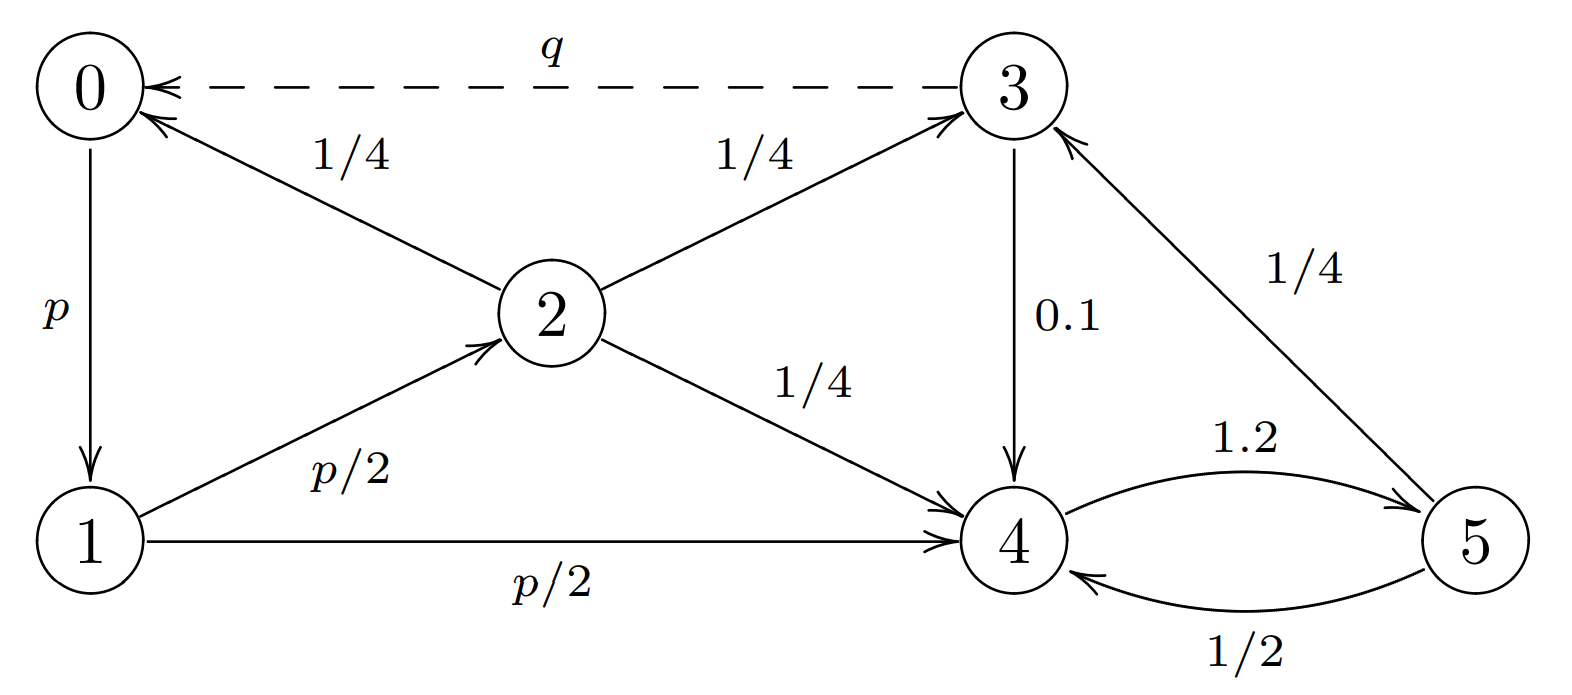
\includegraphics[scale=0.5]{../figures/chain}
	\end{figure}
	
	(se asuma que en cada estado hay una flecha hasta el mismo estado que
	hace que la suma de las probabilidades en salida sea 1), con
	\(p = 0.3\).
	
	\(i)\) Determinar la matriz de transición de la cadena.
	
\end{enunciado}



    Obtenemos la matriz de transición consultando el grafo anterior y
colocando en la posición \(i,j\) la probabilidad de transición del
estado \(i\) al \(j\). En la diagonal colocamos la probabilidad de
mantenernos en el estado \(i,i\), siendo esta \(1\) menos las la suma de
las probabilidades de salir de dicho estado.

\[
    P = 
    \begin{pmatrix}
        1-p & p & 0 & 0 & 0 & 0 \\
        0 & 1-p & p/2 & 0 & p/2 & 0 & \\
        1/4 & 0 & 1/4 & 1/4 & 1/4 & 0 \\
        q & 0 & 0 & 0.9-q & 0.1 & 0 \\
        0 & 0 & 0 & 0 & 1/2 & 1/2 \\
        0 & 0 & 0 & 1/4 & 1/2 & 1/4
    \end{pmatrix}
\]

Como medida de comprobación podemos asegurarnos de que todas las filas
sumen \(1\), como hacen.

\begin{enunciado}
	
	\(ii)\) Simular el funcionamiento de la cadena y hacer una estimación de
	conjunto de \(h_0^2\) y \(h_0^5\) para \(q = 0.1\) y \(q = 0\).
	
\end{enunciado}

    Explicaremos la implementación de la simulación paso a paso. En primer
lugar, creamos una función sencilla que, dados \(p\) y \(q\), devuelve
la matriz \(P\) de nuestro problema.

A continuación definimos una función `collapsa' un estado de nuestro
sistema a un único \(m \in M\). Por ejemplo, dado el estado
\(\phi = [1/3, 2/3]\):

\[ 
collapse(\phi) = 
\begin{cases}
[1, 0] & \quad \text{with probability} \; 1/3 \\
[0, 1] & \quad \text{with probability} \; 2/3
\end{cases}
\]

Para ello utilizaremos que los vectores de estados han de sumar 1 y
aplicaremos el método de la función inversa para elegir a qué estado
colapsar. Esto es, la suma acumulativa de los valores del vector y
generamos un valor uniformemente en \((0,1)\). Comparamos con los
valores de dicha suma acumulativa para ver a qué estado colapsar. Por
ejemplo, para el caso anterior:

    \begin{tcolorbox}[breakable, size=fbox, boxrule=1pt, pad at break*=1mm,colback=cellbackground, colframe=cellborder]
\prompt{In}{incolor}{2}{\boxspacing}
\begin{Verbatim}[commandchars=\\\{\}]
\PY{n}{dist} \PY{o}{=} \PY{n}{stats}\PY{o}{.}\PY{n}{norm}
\PY{n}{dist\PYZus{}pdf} \PY{o}{=} \PY{n}{dist}\PY{o}{.}\PY{n}{pdf}
\PY{n}{dist\PYZus{}icdf} \PY{o}{=} \PY{n}{dist}\PY{o}{.}\PY{n}{ppf}
\PY{n}{dist\PYZus{}cdf} \PY{o}{=} \PY{n}{dist}\PY{o}{.}\PY{n}{cdf}

\PY{n}{p} \PY{o}{=} \PY{l+m+mi}{1}\PY{o}{/}\PY{l+m+mi}{3}
\PY{n}{x} \PY{o}{=} \PY{n}{np}\PY{o}{.}\PY{n}{array}\PY{p}{(}\PY{p}{[}\PY{o}{\PYZhy{}}\PY{l+m+mi}{1}\PY{p}{,} \PY{l+m+mi}{0}\PY{p}{,} \PY{l+m+mi}{1}\PY{p}{,} \PY{l+m+mi}{2}\PY{p}{]}\PY{p}{)}
\PY{n}{y} \PY{o}{=} \PY{n}{np}\PY{o}{.}\PY{n}{array}\PY{p}{(}\PY{p}{[}\PY{n}{p}\PY{p}{,} \PY{l+m+mi}{1}\PY{p}{]}\PY{p}{)}
\PY{n}{yn} \PY{o}{=} \PY{n}{np}\PY{o}{.}\PY{n}{insert}\PY{p}{(}\PY{n}{y}\PY{p}{,} \PY{l+m+mi}{0}\PY{p}{,} \PY{l+m+mi}{0}\PY{p}{)}

\PY{k}{with} \PY{n}{plt}\PY{o}{.}\PY{n}{xkcd}\PY{p}{(}\PY{p}{)}\PY{p}{:}
    \PY{n}{plt}\PY{o}{.}\PY{n}{figure}\PY{p}{(}\PY{n}{figsize}\PY{o}{=}\PY{p}{(}\PY{l+m+mi}{10}\PY{p}{,}\PY{l+m+mi}{6}\PY{p}{)}\PY{p}{)}
    \PY{n}{plt}\PY{o}{.}\PY{n}{hlines}\PY{p}{(}\PY{n}{y}\PY{o}{=}\PY{n}{yn}\PY{p}{,} \PY{n}{xmin}\PY{o}{=}\PY{n}{x}\PY{p}{[}\PY{p}{:}\PY{o}{\PYZhy{}}\PY{l+m+mi}{1}\PY{p}{]}\PY{p}{,} \PY{n}{xmax}\PY{o}{=}\PY{n}{x}\PY{p}{[}\PY{l+m+mi}{1}\PY{p}{:}\PY{p}{]}\PY{p}{,} \PY{n}{zorder}\PY{o}{=}\PY{l+m+mi}{1}\PY{p}{)}
    \PY{n}{plt}\PY{o}{.}\PY{n}{vlines}\PY{p}{(}\PY{n}{x}\PY{o}{=}\PY{n}{x}\PY{p}{[}\PY{l+m+mi}{1}\PY{p}{:}\PY{o}{\PYZhy{}}\PY{l+m+mi}{1}\PY{p}{]}\PY{p}{,} \PY{n}{ymin}\PY{o}{=}\PY{n}{yn}\PY{p}{[}\PY{p}{:}\PY{o}{\PYZhy{}}\PY{l+m+mi}{1}\PY{p}{]}\PY{p}{,} \PY{n}{ymax}\PY{o}{=}\PY{n}{yn}\PY{p}{[}\PY{l+m+mi}{1}\PY{p}{:}\PY{p}{]}\PY{p}{,} \PY{n}{linestyle}\PY{o}{=}\PY{l+s+s1}{\PYZsq{}}\PY{l+s+s1}{dashed}\PY{l+s+s1}{\PYZsq{}}\PY{p}{,} \PY{n}{zorder}\PY{o}{=}\PY{l+m+mi}{1}\PY{p}{)}
    
    \PY{n}{plt}\PY{o}{.}\PY{n}{scatter}\PY{p}{(}\PY{n}{x}\PY{p}{[}\PY{l+m+mi}{1}\PY{p}{:}\PY{o}{\PYZhy{}}\PY{l+m+mi}{1}\PY{p}{]}\PY{p}{,} \PY{n}{y}\PY{p}{,} \PY{n}{s}\PY{o}{=}\PY{l+m+mi}{18}\PY{p}{,} \PY{n}{zorder}\PY{o}{=}\PY{l+m+mi}{2}\PY{p}{)}
    \PY{n}{plt}\PY{o}{.}\PY{n}{scatter}\PY{p}{(}\PY{n}{x}\PY{p}{[}\PY{l+m+mi}{1}\PY{p}{:}\PY{o}{\PYZhy{}}\PY{l+m+mi}{1}\PY{p}{]}\PY{p}{,} \PY{n}{yn}\PY{p}{[}\PY{p}{:}\PY{o}{\PYZhy{}}\PY{l+m+mi}{1}\PY{p}{]}\PY{p}{,} \PY{n}{color}\PY{o}{=}\PY{l+s+s1}{\PYZsq{}}\PY{l+s+s1}{white}\PY{l+s+s1}{\PYZsq{}}\PY{p}{,} \PY{n}{s}\PY{o}{=}\PY{l+m+mi}{18}\PY{p}{,} \PY{n}{zorder}\PY{o}{=}\PY{l+m+mi}{2}\PY{p}{)}

    \PY{n}{plt}\PY{o}{.}\PY{n}{axis}\PY{p}{(}\PY{p}{[}\PY{o}{\PYZhy{}}\PY{l+m+mi}{1}\PY{p}{,} \PY{l+m+mi}{2}\PY{p}{,} \PY{o}{\PYZhy{}}\PY{l+m+mf}{0.05}\PY{p}{,} \PY{l+m+mf}{1.1}\PY{p}{]}\PY{p}{)}
    \PY{k}{for} \PY{n}{q}\PY{p}{,} \PY{n}{x\PYZus{}pos} \PY{o+ow}{in} \PY{n+nb}{zip}\PY{p}{(}\PY{p}{[}\PY{l+m+mf}{0.25}\PY{p}{,} \PY{l+m+mf}{0.8}\PY{p}{]}\PY{p}{,} \PY{n}{x}\PY{p}{[}\PY{l+m+mi}{1}\PY{p}{:}\PY{l+m+mi}{3}\PY{p}{]}\PY{p}{)}\PY{p}{:}
        \PY{n}{plt}\PY{o}{.}\PY{n}{arrow}\PY{p}{(}\PY{o}{\PYZhy{}}\PY{l+m+mi}{1}\PY{p}{,} \PY{n}{q}\PY{p}{,} \PY{l+m+mf}{0.9}\PY{o}{+}\PY{n}{x\PYZus{}pos}\PY{p}{,} \PY{l+m+mi}{0}\PY{p}{,} \PY{n}{head\PYZus{}width}\PY{o}{=}\PY{l+m+mf}{0.05}\PY{p}{,} \PY{n}{head\PYZus{}length}\PY{o}{=}\PY{l+m+mf}{0.1}\PY{p}{,} \PY{n}{fc}\PY{o}{=}\PY{l+s+s1}{\PYZsq{}}\PY{l+s+s1}{b}\PY{l+s+s1}{\PYZsq{}}\PY{p}{,} \PY{n}{ec}\PY{o}{=}\PY{l+s+s1}{\PYZsq{}}\PY{l+s+s1}{b}\PY{l+s+s1}{\PYZsq{}}\PY{p}{)}
        \PY{n}{plt}\PY{o}{.}\PY{n}{arrow}\PY{p}{(}\PY{n}{x\PYZus{}pos}\PY{o}{+}\PY{l+m+mf}{0.05}\PY{p}{,} \PY{n}{q}\PY{p}{,} \PY{l+m+mi}{0}\PY{p}{,} \PY{o}{\PYZhy{}}\PY{n}{q}\PY{o}{+}\PY{l+m+mf}{0.05}\PY{p}{,} \PY{n}{head\PYZus{}width}\PY{o}{=}\PY{l+m+mf}{0.1}\PY{p}{,} \PY{n}{head\PYZus{}length}\PY{o}{=}\PY{l+m+mf}{0.05}\PY{p}{,} \PY{n}{fc}\PY{o}{=}\PY{l+s+s1}{\PYZsq{}}\PY{l+s+s1}{b}\PY{l+s+s1}{\PYZsq{}}\PY{p}{,} \PY{n}{ec}\PY{o}{=}\PY{l+s+s1}{\PYZsq{}}\PY{l+s+s1}{b}\PY{l+s+s1}{\PYZsq{}}\PY{p}{)}

    \PY{n}{plt}\PY{o}{.}\PY{n}{ylabel}\PY{p}{(}\PY{l+s+s1}{\PYZsq{}}\PY{l+s+s1}{1: Generate  U(0,1)}\PY{l+s+s1}{\PYZsq{}}\PY{p}{)}
    \PY{n}{plt}\PY{o}{.}\PY{n}{xlabel}\PY{p}{(}\PY{l+s+s1}{\PYZsq{}}\PY{l+s+s1}{2: Find the inverse CDF}\PY{l+s+s1}{\PYZsq{}}\PY{p}{)}
    \PY{n}{plt}\PY{o}{.}\PY{n}{title}\PY{p}{(}\PY{l+s+s1}{\PYZsq{}}\PY{l+s+s1}{Inverse transform method applied to [1/3, 2/3]}\PY{l+s+s1}{\PYZsq{}}\PY{p}{)}
\end{Verbatim}
\end{tcolorbox}

    \begin{center}
    \adjustimage{max size={0.9\linewidth}{0.9\paperheight}}{output_7_0.png}
    \end{center}
    { \hspace*{\fill} \\}
    
    Implementamos las funciones descritas.

    \begin{tcolorbox}[breakable, size=fbox, boxrule=1pt, pad at break*=1mm,colback=cellbackground, colframe=cellborder]
\prompt{In}{incolor}{3}{\boxspacing}
\begin{Verbatim}[commandchars=\\\{\}]
\PY{k}{def} \PY{n+nf}{get\PYZus{}P}\PY{p}{(}\PY{n}{p}\PY{p}{,} \PY{n}{q}\PY{p}{)}\PY{p}{:}
    \PY{k}{return} \PY{n}{np}\PY{o}{.}\PY{n}{array}\PY{p}{(}\PY{p}{[}\PY{p}{[}  \PY{l+m+mi}{1}\PY{o}{\PYZhy{}}\PY{n}{p}\PY{p}{,}    \PY{n}{p}\PY{p}{,}    \PY{l+m+mf}{0.0}\PY{p}{,}    \PY{l+m+mf}{0.0}\PY{p}{,}    \PY{l+m+mf}{0.0}\PY{p}{,}    \PY{l+m+mf}{0.0}\PY{p}{]}\PY{p}{,}
                    \PY{p}{[}  \PY{l+m+mf}{0.0}\PY{p}{,}  \PY{l+m+mi}{1}\PY{o}{\PYZhy{}}\PY{n}{p}\PY{p}{,}  \PY{n}{p}\PY{o}{/}\PY{l+m+mf}{2.0}\PY{p}{,}    \PY{l+m+mf}{0.0}\PY{p}{,}   \PY{n}{p}\PY{o}{/}\PY{l+m+mf}{2.0}\PY{p}{,}   \PY{l+m+mf}{0.0}\PY{p}{]}\PY{p}{,}
                    \PY{p}{[}\PY{l+m+mi}{1}\PY{o}{/}\PY{l+m+mf}{4.0}\PY{p}{,}  \PY{l+m+mf}{0.0}\PY{p}{,}  \PY{l+m+mi}{1}\PY{o}{/}\PY{l+m+mf}{4.0}\PY{p}{,}   \PY{l+m+mi}{1}\PY{o}{/}\PY{l+m+mf}{4.0}\PY{p}{,}  \PY{l+m+mi}{1}\PY{o}{/}\PY{l+m+mf}{4.0}\PY{p}{,}   \PY{l+m+mf}{0.0}\PY{p}{]}\PY{p}{,}
                    \PY{p}{[}    \PY{n}{q}\PY{p}{,}  \PY{l+m+mf}{0.0}\PY{p}{,}    \PY{l+m+mf}{0.0}\PY{p}{,} \PY{l+m+mi}{1}\PY{o}{\PYZhy{}}\PY{n}{q}\PY{o}{\PYZhy{}}\PY{l+m+mf}{0.1}\PY{p}{,}    \PY{l+m+mf}{0.1}\PY{p}{,}   \PY{l+m+mf}{0.0}\PY{p}{]}\PY{p}{,}
                    \PY{p}{[}  \PY{l+m+mf}{0.0}\PY{p}{,}  \PY{l+m+mf}{0.0}\PY{p}{,}    \PY{l+m+mf}{0.0}\PY{p}{,}     \PY{l+m+mf}{0.0}\PY{p}{,}  \PY{l+m+mi}{1}\PY{o}{/}\PY{l+m+mf}{2.0}\PY{p}{,} \PY{l+m+mi}{1}\PY{o}{/}\PY{l+m+mf}{2.0}\PY{p}{]}\PY{p}{,}
                    \PY{p}{[}  \PY{l+m+mf}{0.0}\PY{p}{,}  \PY{l+m+mf}{0.0}\PY{p}{,}    \PY{l+m+mf}{0.0}\PY{p}{,}    \PY{l+m+mi}{1}\PY{o}{/}\PY{l+m+mf}{4.0}\PY{p}{,} \PY{l+m+mi}{1}\PY{o}{/}\PY{l+m+mf}{2.0}\PY{p}{,} \PY{l+m+mi}{1}\PY{o}{/}\PY{l+m+mf}{4.0}\PY{p}{]}
                    \PY{p}{]}\PY{p}{)}

\PY{k}{def} \PY{n+nf}{collapse}\PY{p}{(}\PY{n}{state}\PY{p}{)}\PY{p}{:}
    \PY{l+s+sd}{\PYZdq{}\PYZdq{}\PYZdq{}}
\PY{l+s+sd}{        Given a state, collapses it to a single position}
\PY{l+s+sd}{        with the given probabilities in the state. For example, given:}
\PY{l+s+sd}{            state = [1/3, 2/3]}
\PY{l+s+sd}{        collapse(state) will output:}
\PY{l+s+sd}{        \PYZhy{} [1, 0] with probability 1/3}
\PY{l+s+sd}{        \PYZhy{} [0, 1] with probability 2/3}
\PY{l+s+sd}{    \PYZdq{}\PYZdq{}\PYZdq{}}
    \PY{n}{F\PYZus{}n} \PY{o}{=} \PY{n}{np}\PY{o}{.}\PY{n}{cumsum}\PY{p}{(}\PY{n}{state}\PY{p}{)}
    \PY{n}{F\PYZus{}n} \PY{o}{=} \PY{n}{np}\PY{o}{.}\PY{n}{insert}\PY{p}{(}\PY{n}{F\PYZus{}n}\PY{p}{,} \PY{l+m+mi}{0}\PY{p}{,} \PY{l+m+mi}{0}\PY{p}{,} \PY{n}{axis}\PY{o}{=}\PY{l+m+mi}{0}\PY{p}{)}
    \PY{n}{r} \PY{o}{=} \PY{n}{random}\PY{o}{.}\PY{n}{uniform}\PY{p}{(}\PY{l+m+mi}{0}\PY{p}{,} \PY{l+m+mi}{1}\PY{p}{)}
    \PY{n}{collapsed} \PY{o}{=} \PY{n}{np}\PY{o}{.}\PY{n}{zeros}\PY{p}{(}\PY{n+nb}{len}\PY{p}{(}\PY{n}{state}\PY{p}{)}\PY{p}{)}
    \PY{k}{for} \PY{n}{i}\PY{p}{,} \PY{p}{(}\PY{n}{x1}\PY{p}{,} \PY{n}{x2}\PY{p}{)} \PY{o+ow}{in} \PY{n+nb}{enumerate}\PY{p}{(}\PY{n+nb}{zip}\PY{p}{(}\PY{n}{F\PYZus{}n}\PY{p}{[}\PY{p}{:}\PY{o}{\PYZhy{}}\PY{l+m+mi}{1}\PY{p}{]}\PY{p}{,} \PY{n}{F\PYZus{}n}\PY{p}{[}\PY{l+m+mi}{1}\PY{p}{:}\PY{p}{]}\PY{p}{)}\PY{p}{)}\PY{p}{:}
        \PY{k}{if} \PY{n}{r} \PY{o}{\PYZgt{}} \PY{n}{x1} \PY{o+ow}{and} \PY{n}{r} \PY{o}{\PYZlt{}} \PY{n}{x2}\PY{p}{:}
            \PY{n}{collapsed}\PY{p}{[}\PY{n}{i}\PY{p}{]} \PY{o}{=} \PY{l+m+mi}{1}
    \PY{k}{return} \PY{n}{collapsed}
\end{Verbatim}
\end{tcolorbox}

    A continuación implementamos la simulación del \textbf{\emph{first
hitting time}} \(H\). Dado un número de pasos \emph{steps}, computamos
del estado actual al siguiente multiplicando por la matriz \(P\) y
colapsamos el estado tras ello. Si quisiéramos obtener el estado de la
simulación tras \(t\) instantes bastaría con multiplicar por \(P^t\) y
colapsar una única vez, pero como hemos de comprobar si hemos alcanzado
el estado objetivo en cada iteración, colapsamos en cada una de ellas.

Finalmente, si trascurridos el número total de pasos no hemos llegado al
estado objetivo, devolveremos \(-1\) simbolizando tiempo infinito.

    \begin{tcolorbox}[breakable, size=fbox, boxrule=1pt, pad at break*=1mm,colback=cellbackground, colframe=cellborder]
\prompt{In}{incolor}{4}{\boxspacing}
\begin{Verbatim}[commandchars=\\\{\}]
\PY{k}{def} \PY{n+nf}{simulate\PYZus{}H}\PY{p}{(}\PY{n}{from\PYZus{}m}\PY{p}{,} \PY{n}{to\PYZus{}m}\PY{p}{,} \PY{n}{P}\PY{p}{,} \PY{n}{steps}\PY{o}{=}\PY{l+m+mi}{10}\PY{o}{*}\PY{o}{*}\PY{l+m+mi}{3}\PY{p}{)}\PY{p}{:}
    \PY{l+s+sd}{\PYZdq{}\PYZdq{}\PYZdq{}}
\PY{l+s+sd}{        Simulate a single random walk through the markov chain}
\PY{l+s+sd}{        described by P and compute the first hitting time from\PYZus{}m to\PYZus{}m.}

\PY{l+s+sd}{        Returns either a natural number if to\PYZus{}m was reached in that time,}
\PY{l+s+sd}{        or \PYZhy{}1 if to\PYZus{}m was never reached/}
\PY{l+s+sd}{    \PYZdq{}\PYZdq{}\PYZdq{}}
    \PY{k}{if} \PY{n}{from\PYZus{}m} \PY{o}{==} \PY{n}{to\PYZus{}m}\PY{p}{:}
        \PY{k}{return} \PY{l+m+mi}{0}

    \PY{n}{state} \PY{o}{=} \PY{n}{np}\PY{o}{.}\PY{n}{zeros}\PY{p}{(}\PY{n+nb}{len}\PY{p}{(}\PY{n}{P}\PY{p}{[}\PY{l+m+mi}{0}\PY{p}{]}\PY{p}{)}\PY{p}{)}
    \PY{n}{state}\PY{p}{[}\PY{n}{from\PYZus{}m}\PY{p}{]} \PY{o}{=} \PY{l+m+mi}{1}

    \PY{k}{for} \PY{n}{step} \PY{o+ow}{in} \PY{n+nb}{range}\PY{p}{(}\PY{l+m+mi}{1}\PY{p}{,} \PY{n}{steps}\PY{o}{+}\PY{l+m+mi}{1}\PY{p}{)}\PY{p}{:}
        \PY{n}{state} \PY{o}{=} \PY{n}{collapse}\PY{p}{(}\PY{n}{state} \PY{o}{@} \PY{n}{P}\PY{p}{)}
        \PY{k}{if} \PY{n}{state}\PY{p}{[}\PY{n}{to\PYZus{}m}\PY{p}{]} \PY{o}{==} \PY{l+m+mi}{1}\PY{p}{:}
            \PY{k}{return} \PY{n}{step}
    \PY{k}{return} \PY{o}{\PYZhy{}}\PY{l+m+mi}{1}
\end{Verbatim}
\end{tcolorbox}

    Pasamos a computar el \textbf{\emph{ever hitting probability}} \(h\).
Para ello lanzaremos la simulación de \(H\) \emph{n\_random\_walks}
veces. Contaremos el número total de veces que alcanzamos el estado
objetivo comprobando que \(H \ge 0\) para obtener la estimación de la
probabilidad buscada.

    \begin{tcolorbox}[breakable, size=fbox, boxrule=1pt, pad at break*=1mm,colback=cellbackground, colframe=cellborder]
\prompt{In}{incolor}{5}{\boxspacing}
\begin{Verbatim}[commandchars=\\\{\}]
\PY{k}{def} \PY{n+nf}{simulate\PYZus{}h}\PY{p}{(}\PY{n}{from\PYZus{}m}\PY{p}{,} \PY{n}{to\PYZus{}m}\PY{p}{,} \PY{n}{P}\PY{p}{,} \PY{n}{steps}\PY{o}{=}\PY{l+m+mi}{10}\PY{o}{*}\PY{o}{*}\PY{l+m+mi}{3}\PY{p}{,} \PY{n}{n\PYZus{}random\PYZus{}walks}\PY{o}{=}\PY{l+m+mi}{10}\PY{o}{*}\PY{o}{*}\PY{l+m+mi}{3}\PY{p}{)}\PY{p}{:}
    \PY{l+s+sd}{\PYZdq{}\PYZdq{}\PYZdq{}}
\PY{l+s+sd}{        Simulate `n\PYZus{}random\PYZus{}walks` random walks through the markov chain}
\PY{l+s+sd}{        described by P and estimate the hitting from\PYZus{}m to\PYZus{}m.}

\PY{l+s+sd}{        Returns the estimation of the probability of hitting from\PYZus{}m}
\PY{l+s+sd}{        to\PYZus{}m in `steps` steps.}
\PY{l+s+sd}{    \PYZdq{}\PYZdq{}\PYZdq{}}
    \PY{n}{total\PYZus{}hits} \PY{o}{=} \PY{l+m+mi}{0}
    \PY{k}{for} \PY{n}{\PYZus{}} \PY{o+ow}{in} \PY{n+nb}{range}\PY{p}{(}\PY{n}{n\PYZus{}random\PYZus{}walks}\PY{p}{)}\PY{p}{:}
        \PY{n}{total\PYZus{}hits} \PY{o}{+}\PY{o}{=} \PY{l+m+mi}{1} \PY{o}{+} \PY{n+nb}{min}\PY{p}{(}\PY{l+m+mi}{0}\PY{p}{,} \PY{n}{simulate\PYZus{}H}\PY{p}{(}\PY{n}{from\PYZus{}m}\PY{o}{=}\PY{n}{from\PYZus{}m}\PY{p}{,} \PY{n}{to\PYZus{}m}\PY{o}{=}\PY{n}{to\PYZus{}m}\PY{p}{,} \PY{n}{P}\PY{o}{=}\PY{n}{P}\PY{p}{,} \PY{n}{steps}\PY{o}{=}\PY{n}{steps}\PY{p}{)}\PY{p}{)}
    \PY{k}{return} \PY{n}{total\PYZus{}hits} \PY{o}{/} \PY{n}{n\PYZus{}random\PYZus{}walks}

\PY{k}{def} \PY{n+nf}{simulate\PYZus{}h\PYZus{}specific}\PY{p}{(}\PY{n}{from\PYZus{}m}\PY{p}{,} \PY{n}{to\PYZus{}m}\PY{p}{,} \PY{n}{p}\PY{o}{=}\PY{l+m+mf}{0.3}\PY{p}{,} \PY{n}{q}\PY{o}{=}\PY{l+m+mf}{0.1}\PY{p}{,} \PY{n}{steps}\PY{o}{=}\PY{l+m+mi}{10}\PY{o}{*}\PY{o}{*}\PY{l+m+mi}{3}\PY{p}{,} \PY{n}{n\PYZus{}random\PYZus{}walks}\PY{o}{=}\PY{l+m+mi}{10}\PY{o}{*}\PY{o}{*}\PY{l+m+mi}{3}\PY{p}{)}\PY{p}{:}
    \PY{n}{P} \PY{o}{=} \PY{n}{get\PYZus{}P}\PY{p}{(}\PY{n}{p}\PY{p}{,} \PY{n}{q}\PY{p}{)}
    \PY{n}{prob} \PY{o}{=} \PY{n}{simulate\PYZus{}h}\PY{p}{(}\PY{n}{from\PYZus{}m}\PY{o}{=}\PY{n}{from\PYZus{}m}\PY{p}{,} \PY{n}{to\PYZus{}m}\PY{o}{=}\PY{n}{to\PYZus{}m}\PY{p}{,} \PY{n}{P}\PY{o}{=}\PY{n}{P}\PY{p}{,} \PY{n}{steps}\PY{o}{=}\PY{n}{steps}\PY{p}{,} \PY{n}{n\PYZus{}random\PYZus{}walks}\PY{o}{=}\PY{n}{n\PYZus{}random\PYZus{}walks}\PY{p}{)}
    \PY{n+nb}{print}\PY{p}{(}\PY{l+s+s1}{\PYZsq{}}\PY{l+s+s1}{(q=}\PY{l+s+si}{\PYZob{}\PYZcb{}}\PY{l+s+s1}{) \PYZhy{} Simulated h}\PY{l+s+si}{\PYZob{}\PYZcb{}}\PY{l+s+si}{\PYZob{}\PYZcb{}}\PY{l+s+s1}{ = }\PY{l+s+si}{\PYZob{}\PYZcb{}}\PY{l+s+s1}{\PYZsq{}}\PY{o}{.}\PY{n}{format}\PY{p}{(}\PY{n}{q}\PY{p}{,} \PY{n}{from\PYZus{}m}\PY{p}{,} \PY{n}{to\PYZus{}m}\PY{p}{,} \PY{n}{prob}\PY{p}{)}\PY{p}{)}
\end{Verbatim}
\end{tcolorbox}

    Veamos los resultados obtenidos para los valores buscados en el
enunciado:

    \begin{tcolorbox}[breakable, size=fbox, boxrule=1pt, pad at break*=1mm,colback=cellbackground, colframe=cellborder]
\prompt{In}{incolor}{6}{\boxspacing}
\begin{Verbatim}[commandchars=\\\{\}]
\PY{n}{random}\PY{o}{.}\PY{n}{seed}\PY{p}{(}\PY{l+m+mi}{123}\PY{p}{)}
\PY{n}{simulate\PYZus{}h\PYZus{}specific}\PY{p}{(}\PY{n}{from\PYZus{}m}\PY{o}{=}\PY{l+m+mi}{0}\PY{p}{,} \PY{n}{to\PYZus{}m}\PY{o}{=}\PY{l+m+mi}{2}\PY{p}{,} \PY{n}{q}\PY{o}{=}\PY{l+m+mf}{0.1}\PY{p}{)}
\PY{n}{simulate\PYZus{}h\PYZus{}specific}\PY{p}{(}\PY{n}{from\PYZus{}m}\PY{o}{=}\PY{l+m+mi}{0}\PY{p}{,} \PY{n}{to\PYZus{}m}\PY{o}{=}\PY{l+m+mi}{5}\PY{p}{,} \PY{n}{q}\PY{o}{=}\PY{l+m+mf}{0.1}\PY{p}{)}
\PY{n}{simulate\PYZus{}h\PYZus{}specific}\PY{p}{(}\PY{n}{from\PYZus{}m}\PY{o}{=}\PY{l+m+mi}{0}\PY{p}{,} \PY{n}{to\PYZus{}m}\PY{o}{=}\PY{l+m+mi}{2}\PY{p}{,} \PY{n}{q}\PY{o}{=}\PY{l+m+mi}{0}\PY{p}{)}
\PY{n}{simulate\PYZus{}h\PYZus{}specific}\PY{p}{(}\PY{n}{from\PYZus{}m}\PY{o}{=}\PY{l+m+mi}{0}\PY{p}{,} \PY{n}{to\PYZus{}m}\PY{o}{=}\PY{l+m+mi}{5}\PY{p}{,} \PY{n}{q}\PY{o}{=}\PY{l+m+mi}{0}\PY{p}{)}
\end{Verbatim}
\end{tcolorbox}

    \begin{Verbatim}[commandchars=\\\{\}]
(q=0.1) - Simulated h02 = 1.0
(q=0.1) - Simulated h05 = 1.0
(q=0) - Simulated h02 = 0.497
(q=0) - Simulated h05 = 1.0
    \end{Verbatim}

    Obtenemos probabilidad total en todos los casos excepto para \(h_0^2\),
donde la probabilidad es cercana a \(0.5\). Esto encaja con nuestra
intuición al estudiar el grafo:

\begin{itemize}
\tightlist
\item
  En los casos en los que \(q=0.1\), nos hayamos ante una cadena
  irreducible finita. Aunque estudiaremos esto en detalle al final de
  este documento, sabemos que todos los nodos de una cadena irreducible
  finita son recurrentes, la probabilidad de pasar por ellos infinitas
  veces es \(1\). Por lo tanto, la de pasar una única vez es también
  \(1\).
\item
  Para \(q=0\), \(h_0^5\) también resulta ser 1. Esto se debe a que nos
  encontramos ante un grafo con dos clases comunicantes: una transitoria
  compuesta por \(\{0,1,2\}\); y una cerrada y recurrente compuesta por
  \(\{3,4,5\}\). Al estudiar la probabilidad de llegar a un nodo de la
  clase cerrada en un cadena con dos clases de esta forma, la
  probabilidad de alcanzar el nodo objetivo siempre será \(1\)
  independientemente del nodo inicial.
\item
  Para \(q=0\), \(h_0^2\) dependerá de la probabilidad de llegar a la
  clase cerrada antes de alcanzar el nodo \(2\), que está en la clase
  transitoria. Observando el grafo podemos visualizar como desde el nodo
  \(1\) hay la misma probabilidad de pasar a la \(2\) que a la clase
  cerrada. Es por ello que \(h_0^2\) ha de ser un medio.
\end{itemize}

\begin{enunciado}
	
	\(iii)\) Simular el funcionamiento de la cadena y hacer una estimación
	de conjunto de \(k_0^2\) y \(k_4^2\) para \(q = 0.1\) y \(q = 0\).
	
\end{enunciado}

    Con la implementación de la simulación anterior en mente es sencillo
calcular el \textbf{\emph{mean hitting probability}} \(k\). Para ello
volvemos a simular \(H\) \emph{n\_random\_walks} veces. Si en alguna de
estas simulaciones no alcanzamos el objetivo, diremos que la
probabilidad media estimada es infinito. En caso contrario, computaremos
la media de los valores \(H\) obtenidos.

    \begin{tcolorbox}[breakable, size=fbox, boxrule=1pt, pad at break*=1mm,colback=cellbackground, colframe=cellborder]
\prompt{In}{incolor}{7}{\boxspacing}
\begin{Verbatim}[commandchars=\\\{\}]
\PY{k}{def} \PY{n+nf}{simulate\PYZus{}k}\PY{p}{(}\PY{n}{from\PYZus{}m}\PY{p}{,} \PY{n}{to\PYZus{}m}\PY{p}{,} \PY{n}{P}\PY{p}{,} \PY{n}{steps}\PY{o}{=}\PY{l+m+mi}{10}\PY{o}{*}\PY{o}{*}\PY{l+m+mi}{3}\PY{p}{,} \PY{n}{n\PYZus{}random\PYZus{}walks}\PY{o}{=}\PY{l+m+mi}{10}\PY{o}{*}\PY{o}{*}\PY{l+m+mi}{3}\PY{p}{)}\PY{p}{:}
    \PY{l+s+sd}{\PYZdq{}\PYZdq{}\PYZdq{}}
\PY{l+s+sd}{        Simulate `n\PYZus{}random\PYZus{}walks` random walks through the markov chain}
\PY{l+s+sd}{        described by P and estimate the mean hitting from\PYZus{}m to\PYZus{}m.}

\PY{l+s+sd}{        Returns the estimation of the mean hittim time from\PYZus{}m to\PYZus{}m in `steps` steps.}
\PY{l+s+sd}{        If any of the random walks didn\PYZsq{}t reach to\PYZus{}m, \PYZhy{}1 is returned, meaning}
\PY{l+s+sd}{        the expected time is infinite.}
\PY{l+s+sd}{    \PYZdq{}\PYZdq{}\PYZdq{}}
    \PY{n}{Hs} \PY{o}{=} \PY{p}{[} \PY{n}{simulate\PYZus{}H}\PY{p}{(}\PY{n}{from\PYZus{}m}\PY{o}{=}\PY{n}{from\PYZus{}m}\PY{p}{,} \PY{n}{to\PYZus{}m}\PY{o}{=}\PY{n}{to\PYZus{}m}\PY{p}{,} \PY{n}{P}\PY{o}{=}\PY{n}{P}\PY{p}{,} \PY{n}{steps}\PY{o}{=}\PY{n}{steps}\PY{p}{)} \PY{k}{for} \PY{n}{\PYZus{}} \PY{o+ow}{in} \PY{n+nb}{range}\PY{p}{(}\PY{n}{n\PYZus{}random\PYZus{}walks}\PY{p}{)} \PY{p}{]}
    \PY{k}{return} \PY{o}{\PYZhy{}}\PY{l+m+mi}{1} \PY{k}{if} \PY{o}{\PYZhy{}}\PY{l+m+mi}{1} \PY{o+ow}{in} \PY{n}{Hs} \PY{k}{else} \PY{n}{np}\PY{o}{.}\PY{n}{mean}\PY{p}{(}\PY{n}{Hs}\PY{p}{)}

\PY{k}{def} \PY{n+nf}{simulate\PYZus{}k\PYZus{}specific}\PY{p}{(}\PY{n}{from\PYZus{}m}\PY{p}{,} \PY{n}{to\PYZus{}m}\PY{p}{,} \PY{n}{p}\PY{o}{=}\PY{l+m+mf}{0.3}\PY{p}{,} \PY{n}{q}\PY{o}{=}\PY{l+m+mf}{0.1}\PY{p}{,} \PY{n}{steps}\PY{o}{=}\PY{l+m+mi}{10}\PY{o}{*}\PY{o}{*}\PY{l+m+mi}{3}\PY{p}{,} \PY{n}{n\PYZus{}random\PYZus{}walks}\PY{o}{=}\PY{l+m+mi}{10}\PY{o}{*}\PY{o}{*}\PY{l+m+mi}{3}\PY{p}{)}\PY{p}{:}
    \PY{n}{P} \PY{o}{=} \PY{n}{get\PYZus{}P}\PY{p}{(}\PY{n}{p}\PY{p}{,} \PY{n}{q}\PY{p}{)}
    \PY{n}{prob} \PY{o}{=} \PY{n}{simulate\PYZus{}k}\PY{p}{(}\PY{n}{from\PYZus{}m}\PY{o}{=}\PY{n}{from\PYZus{}m}\PY{p}{,} \PY{n}{to\PYZus{}m}\PY{o}{=}\PY{n}{to\PYZus{}m}\PY{p}{,} \PY{n}{P}\PY{o}{=}\PY{n}{P}\PY{p}{,} \PY{n}{steps}\PY{o}{=}\PY{n}{steps}\PY{p}{,} \PY{n}{n\PYZus{}random\PYZus{}walks}\PY{o}{=}\PY{n}{n\PYZus{}random\PYZus{}walks}\PY{p}{)}
    \PY{n+nb}{print}\PY{p}{(}\PY{l+s+s1}{\PYZsq{}}\PY{l+s+s1}{(q=}\PY{l+s+si}{\PYZob{}\PYZcb{}}\PY{l+s+s1}{) \PYZhy{} Simulated k}\PY{l+s+si}{\PYZob{}\PYZcb{}}\PY{l+s+si}{\PYZob{}\PYZcb{}}\PY{l+s+s1}{ = }\PY{l+s+si}{\PYZob{}\PYZcb{}}\PY{l+s+s1}{\PYZsq{}}\PY{o}{.}\PY{n}{format}\PY{p}{(}\PY{n}{q}\PY{p}{,} \PY{n}{from\PYZus{}m}\PY{p}{,} \PY{n}{to\PYZus{}m}\PY{p}{,} \PY{n}{prob}\PY{p}{)}\PY{p}{)}
\end{Verbatim}
\end{tcolorbox}

    Veamos los resultados obtenidos para los valores buscados en el
enunciado:

    \begin{tcolorbox}[breakable, size=fbox, boxrule=1pt, pad at break*=1mm,colback=cellbackground, colframe=cellborder]
\prompt{In}{incolor}{8}{\boxspacing}
\begin{Verbatim}[commandchars=\\\{\}]
\PY{n}{simulate\PYZus{}k\PYZus{}specific}\PY{p}{(}\PY{n}{from\PYZus{}m}\PY{o}{=}\PY{l+m+mi}{0}\PY{p}{,} \PY{n}{to\PYZus{}m}\PY{o}{=}\PY{l+m+mi}{2}\PY{p}{,} \PY{n}{q}\PY{o}{=}\PY{l+m+mf}{0.1}\PY{p}{)}
\PY{n}{simulate\PYZus{}k\PYZus{}specific}\PY{p}{(}\PY{n}{from\PYZus{}m}\PY{o}{=}\PY{l+m+mi}{4}\PY{p}{,} \PY{n}{to\PYZus{}m}\PY{o}{=}\PY{l+m+mi}{2}\PY{p}{,} \PY{n}{q}\PY{o}{=}\PY{l+m+mf}{0.1}\PY{p}{)}
\PY{n}{simulate\PYZus{}k\PYZus{}specific}\PY{p}{(}\PY{n}{from\PYZus{}m}\PY{o}{=}\PY{l+m+mi}{0}\PY{p}{,} \PY{n}{to\PYZus{}m}\PY{o}{=}\PY{l+m+mi}{2}\PY{p}{,} \PY{n}{q}\PY{o}{=}\PY{l+m+mi}{0}\PY{p}{)}
\PY{n}{simulate\PYZus{}k\PYZus{}specific}\PY{p}{(}\PY{n}{from\PYZus{}m}\PY{o}{=}\PY{l+m+mi}{4}\PY{p}{,} \PY{n}{to\PYZus{}m}\PY{o}{=}\PY{l+m+mi}{2}\PY{p}{,} \PY{n}{q}\PY{o}{=}\PY{l+m+mi}{0}\PY{p}{)}
\end{Verbatim}
\end{tcolorbox}

    \begin{Verbatim}[commandchars=\\\{\}]
(q=0.1) - Simulated k02 = 45.454
(q=0.1) - Simulated k42 = 72.049
(q=0) - Simulated k02 = -1
(q=0) - Simulated k42 = -1
    \end{Verbatim}

    Por un lado, cuando \(q=0\) obtenemos tiempos medios infinitos. Esto
encaja con nuestro marco teórico, pues si hay alguna posibilidad de no
llegar nunca al estado objetivo (como es el caso con una clase abierta y
otra cerrada, el estado objetivo en la abierta), la esperanza del tiempo
de alcanzar dicho nodo será infinito.

Por otro lado, cuando \(q=0.1\) obtenemos un mayor valor estimado para
\(k_4^2\) que para \(k_0^2\). Con un valor tan pequeño de \(q\), salir
del conjunto \(\{3,4,5\}\) es poco probable. Cuando ocurre, pasaremos
por el estado \(2\) con probabilidad \(0.5\) y volveremos a dicho
subconjunto con la misma probabilidad (esto es equivalente al
razonamiento seguido para \(h_0^2\)). Es por ello que si empezamos en el
estado \(0\) llegaremos antes, en media, al objetivo \(2\) que si
empezásemos dentro del conjunto descrito.

\begin{enunciado}
	
	\(iv)\) Usar el sistema de ecuaciones lineares oportuno para determinar
	los valores teóricos correspondientes a las cantidades estimadas y
	comparar con los valores determinados por medio de la simulación.
	
\end{enunciado}

Nota: si una cantidad \(k\) es \(\infty\) la simulación claramente no
puede dar su valor real. Discutir este caso.

    Por el Teorema 3.4 sabemos que el vector de \emph{hitting probabilities}
\(h^A = [h_0^A, \ldots, h_{n-1}^A]\) es la solución minimal no negativa
del siguiente sistema:

\[
\begin{cases}
  h_m^{A} = 1, & m \in A\\
  h_m^{A} = \sum_{n} P_{mn}h_n^{A}, & m \notin A.
\end{cases}
\]

La segunda ecuación -salvo la fila \(m\)- se puede denotar
matricialmente por \(P \cdot h = h\) o equivalentemente por
\((P - \text{Id}) \; h = 0\), donde \(\text{Id}\) denota la matriz
identidad de orden \(n\).

Añadimos al sistema la restricción adicional dada por la expresión
\(h_m^{A} = 1\) si \(m \in A\) sustituyendo las filas con dichos
\(m \in A\) por filas de la identidad: vectores de ceros con un \(1\) en
la posición \(m\). Así mismo, añadimos un \(1\) al vector independiente
(originalmente de ceros) en las posiciones \(m\). De esta forma hemos
codificado la expresión del teorema en un producto de matrices resoluble
por software de cálculo númerico.

Hemos de comentar una caso adicional. Si la matriz \((P - \text{Id})\)
con las debidas alteraciones fuese singular, la solución mínima no
negativa de dicho sistema obtendrá la solución buscada asignando \(0\)
(el menor valor no negativo) a aquellas incógnitas independientes. Este
caso se da cuando la cadena es conexa con más de una clase comunicante,
como veremos al final de este documento.

Implementamos la resolución teórica de este sistema y comprobamos los
resultados obtenidos:

    \begin{tcolorbox}[breakable, size=fbox, boxrule=1pt, pad at break*=1mm,colback=cellbackground, colframe=cellborder]
\prompt{In}{incolor}{9}{\boxspacing}
\begin{Verbatim}[commandchars=\\\{\}]
\PY{k}{def} \PY{n+nf}{theoretical\PYZus{}h}\PY{p}{(}\PY{n}{P}\PY{p}{,} \PY{n}{to\PYZus{}m}\PY{p}{)}\PY{p}{:}
    \PY{n}{n} \PY{o}{=} \PY{n+nb}{len}\PY{p}{(}\PY{n}{P}\PY{p}{[}\PY{l+m+mi}{0}\PY{p}{]}\PY{p}{)}
    \PY{n}{A} \PY{o}{=} \PY{n}{P} \PY{o}{\PYZhy{}} \PY{n}{np}\PY{o}{.}\PY{n}{identity}\PY{p}{(}\PY{n}{n}\PY{p}{)}
    \PY{n}{b} \PY{o}{=} \PY{n}{np}\PY{o}{.}\PY{n}{zeros}\PY{p}{(}\PY{n}{n}\PY{p}{)}
    \PY{n}{b}\PY{p}{[}\PY{n}{to\PYZus{}m}\PY{p}{]} \PY{o}{=} \PY{l+m+mi}{1}
    \PY{n}{A}\PY{p}{[}\PY{n}{to\PYZus{}m}\PY{p}{]} \PY{o}{=} \PY{n}{b}
    \PY{k}{return} \PY{n}{optimize}\PY{o}{.}\PY{n}{nnls}\PY{p}{(}\PY{n}{A}\PY{p}{,} \PY{n}{b}\PY{p}{)}\PY{p}{[}\PY{l+m+mi}{0}\PY{p}{]}

\PY{k}{def} \PY{n+nf}{theorical\PYZus{}h\PYZus{}specific}\PY{p}{(}\PY{n}{from\PYZus{}m}\PY{p}{,} \PY{n}{to\PYZus{}m}\PY{p}{,} \PY{n}{p}\PY{o}{=}\PY{l+m+mf}{0.3}\PY{p}{,} \PY{n}{q}\PY{o}{=}\PY{l+m+mf}{0.1}\PY{p}{)}\PY{p}{:}
    \PY{n}{P} \PY{o}{=} \PY{n}{get\PYZus{}P}\PY{p}{(}\PY{n}{p}\PY{p}{,} \PY{n}{q}\PY{p}{)}
    \PY{n}{result} \PY{o}{=} \PY{n}{theoretical\PYZus{}h}\PY{p}{(}\PY{n}{P}\PY{p}{,} \PY{n}{to\PYZus{}m}\PY{p}{)}
    \PY{n+nb}{print}\PY{p}{(}\PY{l+s+s1}{\PYZsq{}}\PY{l+s+s1}{(q=}\PY{l+s+si}{\PYZob{}\PYZcb{}}\PY{l+s+s1}{) \PYZhy{} Theoretical h}\PY{l+s+si}{\PYZob{}\PYZcb{}}\PY{l+s+si}{\PYZob{}\PYZcb{}}\PY{l+s+s1}{ = }\PY{l+s+si}{\PYZob{}\PYZcb{}}\PY{l+s+s1}{\PYZsq{}}\PY{o}{.}\PY{n}{format}\PY{p}{(}\PY{n}{q}\PY{p}{,} \PY{n}{from\PYZus{}m}\PY{p}{,} \PY{n}{to\PYZus{}m}\PY{p}{,} \PY{n}{result}\PY{p}{[}\PY{n}{from\PYZus{}m}\PY{p}{]}\PY{p}{)}\PY{p}{)}
\end{Verbatim}
\end{tcolorbox}

    \begin{tcolorbox}[breakable, size=fbox, boxrule=1pt, pad at break*=1mm,colback=cellbackground, colframe=cellborder]
\prompt{In}{incolor}{10}{\boxspacing}
\begin{Verbatim}[commandchars=\\\{\}]
\PY{n}{theorical\PYZus{}h\PYZus{}specific}\PY{p}{(}\PY{n}{from\PYZus{}m}\PY{o}{=}\PY{l+m+mi}{0}\PY{p}{,} \PY{n}{to\PYZus{}m}\PY{o}{=}\PY{l+m+mi}{2}\PY{p}{,} \PY{n}{q}\PY{o}{=}\PY{l+m+mf}{0.1}\PY{p}{)}
\PY{n}{theorical\PYZus{}h\PYZus{}specific}\PY{p}{(}\PY{n}{from\PYZus{}m}\PY{o}{=}\PY{l+m+mi}{0}\PY{p}{,} \PY{n}{to\PYZus{}m}\PY{o}{=}\PY{l+m+mi}{5}\PY{p}{,} \PY{n}{q}\PY{o}{=}\PY{l+m+mf}{0.1}\PY{p}{)}
\PY{n}{theorical\PYZus{}h\PYZus{}specific}\PY{p}{(}\PY{n}{from\PYZus{}m}\PY{o}{=}\PY{l+m+mi}{0}\PY{p}{,} \PY{n}{to\PYZus{}m}\PY{o}{=}\PY{l+m+mi}{2}\PY{p}{,} \PY{n}{q}\PY{o}{=}\PY{l+m+mi}{0}\PY{p}{)}
\PY{n}{theorical\PYZus{}h\PYZus{}specific}\PY{p}{(}\PY{n}{from\PYZus{}m}\PY{o}{=}\PY{l+m+mi}{0}\PY{p}{,} \PY{n}{to\PYZus{}m}\PY{o}{=}\PY{l+m+mi}{5}\PY{p}{,} \PY{n}{q}\PY{o}{=}\PY{l+m+mi}{0}\PY{p}{)}
\end{Verbatim}
\end{tcolorbox}

    \begin{Verbatim}[commandchars=\\\{\}]
(q=0.1) - Theoretical h02 = 1.0000000000000007
(q=0.1) - Theoretical h05 = 0.9999999999999981
(q=0) - Theoretical h02 = 0.5
(q=0) - Theoretical h05 = 0.9999999999999986
    \end{Verbatim}

    Los resultados son prácticamente equivalentes a los obtenidos con la
simulación. Al haber utilizado \textbf{\emph{scipy.optimize.nnls}} para
computar la solución al sistema, obtenemos valores muy próximos a la
verdaderamente solución teórica sin ser exactamente iguales.

Pasamos al estudio del \textbf{\emph{mean hitting time}} teórico. Por el
teorema 3.5 sabemos que el vector de \emph{mean hitting times}
\(k^A = [k_0^A, \ldots, k_{n-1}^A]\) es la solución minimal no negativa
del siguiente sistema:

\[
\begin{cases}
  k_m^{A} = 0, & m \in A\\
  k_m^{A} = 1 + \sum_{n} P_{mn}h_n^{A}, & m \notin A.
\end{cases}
\]

De nuevo, la segunda ecuación se traduce en la expresión
\(k = 1 + P \cdot k\). Esto es equivalente a \((\text{Id} - P)k = 1\).
Alteramos esta ecuación añadiendo la primera ecuación del sistema
sustituyendo las filas \(m \in A\) de la matriz anterior por filas de
ceros con un \(1\) en la posición \(m\) y añadiendo un \(0\) en la
respectiva posición del vector independiente. Volveremos a utilizar
\textbf{\emph{scipy.optimize.nnls}} para resolver el sistema.

Hemos de enter en cuenta que si el valor medio es infinito, este sistema
no puede darnos dicho valor. Como sabemos que esto es equivalente a
obtener un valor \(h_m^n < 1\), computaremos este valor en primer lugar
y si es menor \(1\) diremos que \(k_m^n = \infty\).

    \begin{tcolorbox}[breakable, size=fbox, boxrule=1pt, pad at break*=1mm,colback=cellbackground, colframe=cellborder]
\prompt{In}{incolor}{11}{\boxspacing}
\begin{Verbatim}[commandchars=\\\{\}]
\PY{k}{def} \PY{n+nf}{theoretical\PYZus{}k}\PY{p}{(}\PY{n}{P}\PY{p}{,} \PY{n}{to\PYZus{}m}\PY{p}{)}\PY{p}{:}
    \PY{n}{n} \PY{o}{=} \PY{n+nb}{len}\PY{p}{(}\PY{n}{P}\PY{p}{[}\PY{l+m+mi}{0}\PY{p}{]}\PY{p}{)}
    \PY{n}{A} \PY{o}{=} \PY{n}{np}\PY{o}{.}\PY{n}{identity}\PY{p}{(}\PY{n}{n}\PY{p}{)} \PY{o}{\PYZhy{}} \PY{n}{P}
    \PY{n}{b} \PY{o}{=} \PY{n}{np}\PY{o}{.}\PY{n}{ones}\PY{p}{(}\PY{n}{n}\PY{p}{)}
    \PY{n}{b}\PY{p}{[}\PY{n}{to\PYZus{}m}\PY{p}{]} \PY{o}{=} \PY{l+m+mi}{0}
    \PY{n}{A}\PY{p}{[}\PY{n}{to\PYZus{}m}\PY{p}{]} \PY{o}{=} \PY{n}{np}\PY{o}{.}\PY{n}{logical\PYZus{}not}\PY{p}{(}\PY{n}{b}\PY{p}{)}
    \PY{k}{return} \PY{n}{optimize}\PY{o}{.}\PY{n}{nnls}\PY{p}{(}\PY{n}{A}\PY{p}{,} \PY{n}{b}\PY{p}{)}\PY{p}{[}\PY{l+m+mi}{0}\PY{p}{]}

\PY{k}{def} \PY{n+nf}{theorical\PYZus{}k\PYZus{}specific}\PY{p}{(}\PY{n}{from\PYZus{}m}\PY{p}{,} \PY{n}{to\PYZus{}m}\PY{p}{,} \PY{n}{p}\PY{o}{=}\PY{l+m+mf}{0.3}\PY{p}{,} \PY{n}{q}\PY{o}{=}\PY{l+m+mf}{0.1}\PY{p}{)}\PY{p}{:}
    \PY{n}{P} \PY{o}{=} \PY{n}{get\PYZus{}P}\PY{p}{(}\PY{n}{p}\PY{p}{,} \PY{n}{q}\PY{p}{)}
    \PY{n}{h} \PY{o}{=} \PY{n}{theoretical\PYZus{}h}\PY{p}{(}\PY{n}{P}\PY{p}{,} \PY{n}{to\PYZus{}m}\PY{p}{)}\PY{p}{[}\PY{n}{from\PYZus{}m}\PY{p}{]}

    \PY{n}{result} \PY{o}{=} \PY{l+s+s1}{\PYZsq{}}\PY{l+s+s1}{infinity}\PY{l+s+s1}{\PYZsq{}}
    \PY{k}{if} \PY{n}{h} \PY{o}{\PYZgt{}} \PY{l+m+mf}{0.995}\PY{p}{:}
        \PY{n}{result} \PY{o}{=} \PY{n}{theoretical\PYZus{}k}\PY{p}{(}\PY{n}{P}\PY{p}{,} \PY{n}{to\PYZus{}m}\PY{p}{)}\PY{p}{[}\PY{n}{from\PYZus{}m}\PY{p}{]}

    \PY{n+nb}{print}\PY{p}{(}\PY{l+s+s1}{\PYZsq{}}\PY{l+s+s1}{(q=}\PY{l+s+si}{\PYZob{}\PYZcb{}}\PY{l+s+s1}{) \PYZhy{} Theoretical k}\PY{l+s+si}{\PYZob{}\PYZcb{}}\PY{l+s+si}{\PYZob{}\PYZcb{}}\PY{l+s+s1}{ = }\PY{l+s+si}{\PYZob{}\PYZcb{}}\PY{l+s+s1}{\PYZsq{}}\PY{o}{.}\PY{n}{format}\PY{p}{(}\PY{n}{q}\PY{p}{,} \PY{n}{from\PYZus{}m}\PY{p}{,} \PY{n}{to\PYZus{}m}\PY{p}{,} \PY{n}{result}\PY{p}{)}\PY{p}{)}
\end{Verbatim}
\end{tcolorbox}

    Comprobemos los resultados obtenidos:

    \begin{tcolorbox}[breakable, size=fbox, boxrule=1pt, pad at break*=1mm,colback=cellbackground, colframe=cellborder]
\prompt{In}{incolor}{12}{\boxspacing}
\begin{Verbatim}[commandchars=\\\{\}]
\PY{n}{theorical\PYZus{}k\PYZus{}specific}\PY{p}{(}\PY{n}{from\PYZus{}m}\PY{o}{=}\PY{l+m+mi}{0}\PY{p}{,} \PY{n}{to\PYZus{}m}\PY{o}{=}\PY{l+m+mi}{2}\PY{p}{,} \PY{n}{q}\PY{o}{=}\PY{l+m+mf}{0.1}\PY{p}{)}
\PY{n}{theorical\PYZus{}k\PYZus{}specific}\PY{p}{(}\PY{n}{from\PYZus{}m}\PY{o}{=}\PY{l+m+mi}{4}\PY{p}{,} \PY{n}{to\PYZus{}m}\PY{o}{=}\PY{l+m+mi}{2}\PY{p}{,} \PY{n}{q}\PY{o}{=}\PY{l+m+mf}{0.1}\PY{p}{)}
\PY{n}{theorical\PYZus{}k\PYZus{}specific}\PY{p}{(}\PY{n}{from\PYZus{}m}\PY{o}{=}\PY{l+m+mi}{0}\PY{p}{,} \PY{n}{to\PYZus{}m}\PY{o}{=}\PY{l+m+mi}{2}\PY{p}{,} \PY{n}{q}\PY{o}{=}\PY{l+m+mi}{0}\PY{p}{)}
\PY{n}{theorical\PYZus{}k\PYZus{}specific}\PY{p}{(}\PY{n}{from\PYZus{}m}\PY{o}{=}\PY{l+m+mi}{4}\PY{p}{,} \PY{n}{to\PYZus{}m}\PY{o}{=}\PY{l+m+mi}{2}\PY{p}{,} \PY{n}{q}\PY{o}{=}\PY{l+m+mi}{0}\PY{p}{)}
\end{Verbatim}
\end{tcolorbox}

    \begin{Verbatim}[commandchars=\\\{\}]
(q=0.1) - Theoretical k02 = 43.33333333333339
(q=0.1) - Theoretical k42 = 73.33333333333343
(q=0) - Theoretical k02 = infinity
(q=0) - Theoretical k42 = infinity
    \end{Verbatim}

    De nuevo, estos resultados encajan con los valores obtenidos en la
simulación.

\begin{enunciado}
	
	\(v)\) Para el caso \(q = 0.1\), dibujar el grafico de
	\(g(t) = P[H_0^{\{4\}} = t]\)
	
\end{enunciado}

    Para estimar \(g(t)\) realizaremos un número elevado de simulaciones de
\(H_0^4\), \emph{n\_simulations}. Estimamos \(g(t)\) por el cociente de
el número de ejecuciones que terminaron en tiempo \(t\) entre el número
de simulaciones. Por el estudio realizado en los apartados anteriores
sabemos que \(h_0^4 = 1\) (nos hayamos ante una cadena irreducible), por
lo que no hemos de preocuparnos de no llegar nunca al nodo \(4\). En
particular, la gran mayoría de ejecuciones llegan en tiempos inferiores
a \(40\).

    \begin{tcolorbox}[breakable, size=fbox, boxrule=1pt, pad at break*=1mm,colback=cellbackground, colframe=cellborder]
\prompt{In}{incolor}{13}{\boxspacing}
\begin{Verbatim}[commandchars=\\\{\}]
\PY{k}{def} \PY{n+nf}{plot\PYZus{}g}\PY{p}{(}\PY{n}{p}\PY{o}{=}\PY{l+m+mf}{0.3}\PY{p}{,} \PY{n}{q}\PY{o}{=}\PY{l+m+mf}{0.1}\PY{p}{,} \PY{n}{from\PYZus{}m}\PY{o}{=}\PY{l+m+mi}{0}\PY{p}{,} \PY{n}{to\PYZus{}m}\PY{o}{=}\PY{l+m+mi}{4}\PY{p}{,} \PY{n}{max\PYZus{}steps}\PY{o}{=}\PY{l+m+mi}{100}\PY{p}{,} \PY{n}{n\PYZus{}simulations}\PY{o}{=}\PY{l+m+mi}{10}\PY{o}{*}\PY{o}{*}\PY{l+m+mi}{5}\PY{p}{)}\PY{p}{:}
    \PY{n}{P} \PY{o}{=} \PY{n}{get\PYZus{}P}\PY{p}{(}\PY{n}{p}\PY{p}{,} \PY{n}{q}\PY{p}{)}

    \PY{n}{Hs} \PY{o}{=} \PY{p}{[} \PY{n}{simulate\PYZus{}H}\PY{p}{(}\PY{n}{from\PYZus{}m}\PY{o}{=}\PY{n}{from\PYZus{}m}\PY{p}{,} \PY{n}{to\PYZus{}m}\PY{o}{=}\PY{n}{to\PYZus{}m}\PY{p}{,} \PY{n}{P}\PY{o}{=}\PY{n}{P}\PY{p}{,} \PY{n}{steps}\PY{o}{=}\PY{n}{max\PYZus{}steps}\PY{p}{)} \PY{k}{for} \PY{n}{\PYZus{}} \PY{o+ow}{in} \PY{n+nb}{range}\PY{p}{(}\PY{n}{n\PYZus{}simulations}\PY{p}{)} \PY{p}{]}
    \PY{n}{counted} \PY{o}{=} \PY{n}{defaultdict}\PY{p}{(}\PY{n+nb}{int}\PY{p}{,} \PY{n+nb}{dict}\PY{p}{(}\PY{n}{Counter}\PY{p}{(}\PY{n}{Hs}\PY{p}{)}\PY{p}{)}\PY{p}{)}
    \PY{n}{y} \PY{o}{=} \PY{n}{np}\PY{o}{.}\PY{n}{array}\PY{p}{(}\PY{p}{[} \PY{n}{counted}\PY{p}{[}\PY{n}{i}\PY{p}{]} \PY{k}{for} \PY{n}{i} \PY{o+ow}{in} \PY{n+nb}{range}\PY{p}{(}\PY{n}{max\PYZus{}steps}\PY{p}{)} \PY{p}{]}\PY{p}{)} \PY{o}{/} \PY{n}{n\PYZus{}simulations}
    
    \PY{n}{plt}\PY{o}{.}\PY{n}{figure}\PY{p}{(}\PY{n}{figsize}\PY{o}{=}\PY{p}{(}\PY{l+m+mi}{12}\PY{p}{,} \PY{l+m+mi}{8}\PY{p}{)}\PY{p}{)}
    \PY{n}{plt}\PY{o}{.}\PY{n}{plot}\PY{p}{(}\PY{n+nb}{list}\PY{p}{(}\PY{n+nb}{range}\PY{p}{(}\PY{n}{max\PYZus{}steps}\PY{p}{)}\PY{p}{)}\PY{p}{,} \PY{n}{y}\PY{p}{)}
    \PY{n}{plt}\PY{o}{.}\PY{n}{xlabel}\PY{p}{(}\PY{l+s+s1}{\PYZsq{}}\PY{l+s+s1}{Time (t, discrete)}\PY{l+s+s1}{\PYZsq{}}\PY{p}{)}
    \PY{n}{plt}\PY{o}{.}\PY{n}{ylabel}\PY{p}{(}\PY{l+s+s1}{\PYZsq{}}\PY{l+s+s1}{g(t)}\PY{l+s+s1}{\PYZsq{}}\PY{p}{)}
    \PY{n}{plt}\PY{o}{.}\PY{n}{title}\PY{p}{(}\PY{l+s+s1}{\PYZsq{}}\PY{l+s+s1}{First hitting time from 0 to 4}\PY{l+s+s1}{\PYZsq{}}\PY{p}{)}
    \PY{n}{plt}\PY{o}{.}\PY{n}{show}\PY{p}{(}\PY{p}{)}

\PY{n}{plot\PYZus{}g}\PY{p}{(}\PY{p}{)}
\end{Verbatim}
\end{tcolorbox}

    \begin{center}
    \adjustimage{max size={0.9\linewidth}{0.9\paperheight}}{output_34_0.png}
    \end{center}
    { \hspace*{\fill} \\}
    
    Por un lado, merece la pena comentar el pequeño delay inicial: ninguna
ejecución llega al estado \(4\) en menos de dos instantes. Mirando el
grafo de nuestra cadena, este resultado es obvio: el menor camino de
\(0\) a \(4\) tiene longitud \(2\). Conforme el tiempo aumenta, la
mayoría de caminantes aleatorios que estaban todavía en los estados
\(0\), \(1\) y \(2\) acaban llegando al conjunto \(\{3,4\}\), terminando
en su mayoría en dicho estado.

Recordemos que por la configuración de nuestra cadena, siempre podemos
tardar un tiempo arbitrariamente alto en alcanzar este estado, aunque la
probabilidad sea muy pequeña.

Por otro lado, merece la pena comentar que no observamos ningún tipo de
periodicidad en esta gráfica. Por ejemplo, si nos encontrásemos ante un
gráfico bipartido, únicamente podríamos llegar a cada estado en los
tiempos pares o impares, pero no en ambos. Si nos encontrásemos antes un
grafo tripartido, sólo podríamos llegar cada 3 tiempos. Este no es el
caso en nuestra cadena.


\begin{enunciado}
	
	\(vi)\) Razonar si \(H_0^{\{4\}} < H_0^{\{5\}}\).
	
\end{enunciado}

    En efecto. Intuitivamente este resultado es obvio: no podemos llegar al
nodo \(5\) sin pasar por el \(4\), así que el tiempo mínimo de llegada
al nodo \(5\) siempre será 1 instante superior.

\section*{Resultados adicionales}

Enunciamos a continuación una serie de resultados asociados a la teoría de cadenas de Markov que puede ayudarnos a ganar intuición.

Sean $C_1, C_2$ dos clases comunicantes. Si existen un camino de $C_1$ a $C_2$ y viceversa, entonces son la misma clase de Markov. Esto nos indica que la cadena reducida en la que representamos únicamente las clases comunicantes ha de ser un árbol.

Si colocamos los nodos raíz del árbol -aquellos a los que no llega ninguna arista del grafo- en la parte superior del diagrama y pintamos todos los enlaces hacia abajo en una estructura "de cascada" los siguientes resultados se vuelven muy intuitivos:

\begin{itemize}
	\item Las clases cerradas son aquellas situadas en la parte inferior de dicha cascada, aquellas de las que no sale ninguna arista.
	\item Las clases abiertas son las superiores, de las que salen aristas. Con esta visión en mente es sencillo darse cuenta de que \textbf{una clase es transitiva si y sólo si es abierta}.
	\item Si hay posibles estados ($|M| \ \infty$), puede haber infinitas clases abiertas y/o cerradas. Puede incluso no haber ninguna clase cerrada. Además, una cerrada y finita siempre será recurrente, pero el recíproco no es cierto como vimos en clase.
	\item Si hay únicamente una clase comunicante, la cadena es irredubile, y dicha clase será cerrada. De nuevo, si es finita será también recurrente pero el recíproco no podemos asegurarlo. Este es el caso de nuestro grafo si $q=0.1$: la cadena es irreducible y finita. Por lo tanto, $h_m^n = 1$ sin necesidad de hacer ninguna cuenta adicional.
	\item El caso que estudiaremos con mayor frecuencia es el de una cadena finita con más de una clase. En este caso \textbf{siempre podemos asegurar la existencia de una clase cerrada y recurrente}: Si no la hubiese, habría un ciclo en el grafo y la cadena sería irreducible. Además, si la cadena es conexa habrá también al menos una cadena abierta.
\end{itemize}

\end{document}
